\documentclass[
  jou,
  floatsintext,
  longtable,
  a4paper,
  nolmodern,
  notxfonts,
  notimes,
  colorlinks=true,linkcolor=blue,citecolor=blue,urlcolor=blue]{apa7}

\usepackage{amsmath}
\usepackage{amssymb}



\usepackage[bidi=default]{babel}
\babelprovide[main,import]{spanish}


\babelfont{rm}[,RawFeature={fallback=mainfontfallback}]{Latin Modern
Roman}
% get rid of language-specific shorthands (see #6817):
\let\LanguageShortHands\languageshorthands
\def\languageshorthands#1{}

\RequirePackage{longtable}
\RequirePackage{threeparttablex}

\makeatletter
\renewcommand{\paragraph}{\@startsection{paragraph}{4}{\parindent}%
	{0\baselineskip \@plus 0.2ex \@minus 0.2ex}%
	{-.5em}%
	{\normalfont\normalsize\bfseries\typesectitle}}

\renewcommand{\subparagraph}[1]{\@startsection{subparagraph}{5}{0.5em}%
	{0\baselineskip \@plus 0.2ex \@minus 0.2ex}%
	{-\z@\relax}%
	{\normalfont\normalsize\bfseries\itshape\hspace{\parindent}{#1}\textit{\addperi}}{\relax}}
\makeatother




\usepackage{longtable, booktabs, multirow, multicol, colortbl, hhline, caption, array, float, xpatch}
\usepackage{subcaption}


\renewcommand\thesubfigure{\Alph{subfigure}}
\setcounter{topnumber}{2}
\setcounter{bottomnumber}{2}
\setcounter{totalnumber}{4}
\renewcommand{\topfraction}{0.85}
\renewcommand{\bottomfraction}{0.85}
\renewcommand{\textfraction}{0.15}
\renewcommand{\floatpagefraction}{0.7}

\usepackage{tcolorbox}
\tcbuselibrary{listings,theorems, breakable, skins}
\usepackage{fontawesome5}

\definecolor{quarto-callout-color}{HTML}{909090}
\definecolor{quarto-callout-note-color}{HTML}{0758E5}
\definecolor{quarto-callout-important-color}{HTML}{CC1914}
\definecolor{quarto-callout-warning-color}{HTML}{EB9113}
\definecolor{quarto-callout-tip-color}{HTML}{00A047}
\definecolor{quarto-callout-caution-color}{HTML}{FC5300}
\definecolor{quarto-callout-color-frame}{HTML}{ACACAC}
\definecolor{quarto-callout-note-color-frame}{HTML}{4582EC}
\definecolor{quarto-callout-important-color-frame}{HTML}{D9534F}
\definecolor{quarto-callout-warning-color-frame}{HTML}{F0AD4E}
\definecolor{quarto-callout-tip-color-frame}{HTML}{02B875}
\definecolor{quarto-callout-caution-color-frame}{HTML}{FD7E14}

%\newlength\Oldarrayrulewidth
%\newlength\Oldtabcolsep


\usepackage{hyperref}




\providecommand{\tightlist}{%
  \setlength{\itemsep}{0pt}\setlength{\parskip}{0pt}}
\usepackage{longtable,booktabs,array}
\usepackage{calc} % for calculating minipage widths
% Correct order of tables after \paragraph or \subparagraph
\usepackage{etoolbox}
\makeatletter
\patchcmd\longtable{\par}{\if@noskipsec\mbox{}\fi\par}{}{}
\makeatother
% Allow footnotes in longtable head/foot
\IfFileExists{footnotehyper.sty}{\usepackage{footnotehyper}}{\usepackage{footnote}}
\makesavenoteenv{longtable}

\usepackage{graphicx}
\makeatletter
\newsavebox\pandoc@box
\newcommand*\pandocbounded[1]{% scales image to fit in text height/width
  \sbox\pandoc@box{#1}%
  \Gscale@div\@tempa{\textheight}{\dimexpr\ht\pandoc@box+\dp\pandoc@box\relax}%
  \Gscale@div\@tempb{\linewidth}{\wd\pandoc@box}%
  \ifdim\@tempb\p@<\@tempa\p@\let\@tempa\@tempb\fi% select the smaller of both
  \ifdim\@tempa\p@<\p@\scalebox{\@tempa}{\usebox\pandoc@box}%
  \else\usebox{\pandoc@box}%
  \fi%
}
% Set default figure placement to htbp
\def\fps@figure{htbp}
\makeatother







\usepackage{fontspec} 

\defaultfontfeatures{Scale=MatchLowercase}
\defaultfontfeatures[\rmfamily]{Ligatures=TeX,Scale=1}

  \setmainfont[,RawFeature={fallback=mainfontfallback}]{Latin Modern
Roman}




\title{Visualización de Datos con Python: Técnicas y Ejemplos de
Gráficos para Análisis de Datos}


\shorttitle{Visualización con Python}


\usepackage{etoolbox}



\ccoppy{\textcopyright~2025}



\author{Elmer Achalma}



\affiliation{
{Economía, Universidad Nacional de San Cristóbal de Huamanga}}




\leftheader{Achalma}

\date{2025-05-10}


\abstract{Este documento presenta una colección de ejemplos prácticos de
visualización de datos utilizando Python y la biblioteca Matplotlib. Se
incluyen gráficos de líneas, barras, histogramas, circulares, de caja y
combinados, cada uno acompañado de código comentado y optimizado. El
objetivo es proporcionar una guía educativa para estudiantes y
profesionales interesados en representar datos de manera clara y
efectiva, con énfasis en buenas prácticas de diseño y presentación. }

\keywords{Visualización de datos, Python, Matplotlib, Gráficos
estadísticos, Análisis de datos}

\authornote{\par{\addORCIDlink{Elmer Achalma}{0000-0001-6996-3364}} 

\par{   Los autores no tienen conflictos de intereses que
revelar.  Agradezco a mis maestros por su orientación en el aprendizaje
de la programación y visualización de datos, a mis padres por su apoyo
constante durante mi formación, y a Dios por la salud y fortaleza para
perseguir mis metas. Me comprometo a seguir mejorando mis habilidades en
la universidad y en todos los ámbitos, siempre con respeto.  Los roles
de autor se clasificaron utilizando la taxonomía de roles de colaborador
(CRediT; https://credit.niso.org/) de la siguiente manera:  Elmer
Achalma:   Investigación, Programación, Redacción}
\par{La correspondencia relativa a este artículo debe dirigirse a Elmer
Achalma, Email: \href{mailto:elmer.achalma.09@unsch.edu.pe}{elmer.achalma.09@unsch.edu.pe}}
}

\usepackage{pbalance}
% \usepackage{float}
\makeatletter
\let\oldtpt\ThreePartTable
\let\endoldtpt\endThreePartTable
\def\ThreePartTable{\@ifnextchar[\ThreePartTable@i \ThreePartTable@ii}
\def\ThreePartTable@i[#1]{\begin{figure}[!htbp]
\onecolumn
\begin{minipage}{0.485\textwidth}
\oldtpt[#1]
}
\def\ThreePartTable@ii{\begin{figure}[!htbp]
\onecolumn
\begin{minipage}{0.48\textwidth}
\oldtpt
}
\def\endThreePartTable{
\endoldtpt
\end{minipage}
\twocolumn
\end{figure}}
\makeatother


\makeatletter
\let\endoldlt\endlongtable		
\def\endlongtable{
\hline
\endoldlt}
\makeatother

\newenvironment{twocolumntable}% environment name
{% begin code
\begin{table*}[!htbp]%
\onecolumn%
}%
{%
\twocolumn%
\end{table*}%
}% end code

\urlstyle{same}



\makeatletter
\@ifpackageloaded{caption}{}{\usepackage{caption}}
\AtBeginDocument{%
\ifdefined\contentsname
  \renewcommand*\contentsname{Tabla de contenidos}
\else
  \newcommand\contentsname{Tabla de contenidos}
\fi
\ifdefined\listfigurename
  \renewcommand*\listfigurename{List of Figures}
\else
  \newcommand\listfigurename{List of Figures}
\fi
\ifdefined\listtablename
  \renewcommand*\listtablename{List of Tables}
\else
  \newcommand\listtablename{List of Tables}
\fi
\ifdefined\figurename
  \renewcommand*\figurename{Figura}
\else
  \newcommand\figurename{Figura}
\fi
\ifdefined\tablename
  \renewcommand*\tablename{Tabla}
\else
  \newcommand\tablename{Tabla}
\fi
}
\@ifpackageloaded{float}{}{\usepackage{float}}
\floatstyle{ruled}
\@ifundefined{c@chapter}{\newfloat{codelisting}{h}{lop}}{\newfloat{codelisting}{h}{lop}[chapter]}
\floatname{codelisting}{Listing}
\newcommand*\listoflistings{\listof{codelisting}{List of Listings}}
\makeatother
\makeatletter
\makeatother
\makeatletter
\@ifpackageloaded{caption}{}{\usepackage{caption}}
\@ifpackageloaded{subcaption}{}{\usepackage{subcaption}}
\makeatother

% From https://tex.stackexchange.com/a/645996/211326
%%% apa7 doesn't want to add appendix section titles in the toc
%%% let's make it do it
\makeatletter
\xpatchcmd{\appendix}
  {\par}
  {\addcontentsline{toc}{section}{\@currentlabelname}\par}
  {}{}
\makeatother

%% Disable longtable counter
%% https://tex.stackexchange.com/a/248395/211326

\usepackage{etoolbox}

\makeatletter
\patchcmd{\LT@caption}
  {\bgroup}
  {\bgroup\global\LTpatch@captiontrue}
  {}{}
\patchcmd{\longtable}
  {\par}
  {\par\global\LTpatch@captionfalse}
  {}{}
\apptocmd{\endlongtable}
  {\ifLTpatch@caption\else\addtocounter{table}{-1}\fi}
  {}{}
\newif\ifLTpatch@caption
\makeatother

\begin{document}

\maketitle

\hypertarget{toc}{}
\tableofcontents
\newpage
\section[Introduction]{Visualización de Datos con Python}

\setcounter{secnumdepth}{5}

\setlength\LTleft{0pt}


\section{Grafico de lineas}\label{grafico-de-lineas}

\pandocbounded{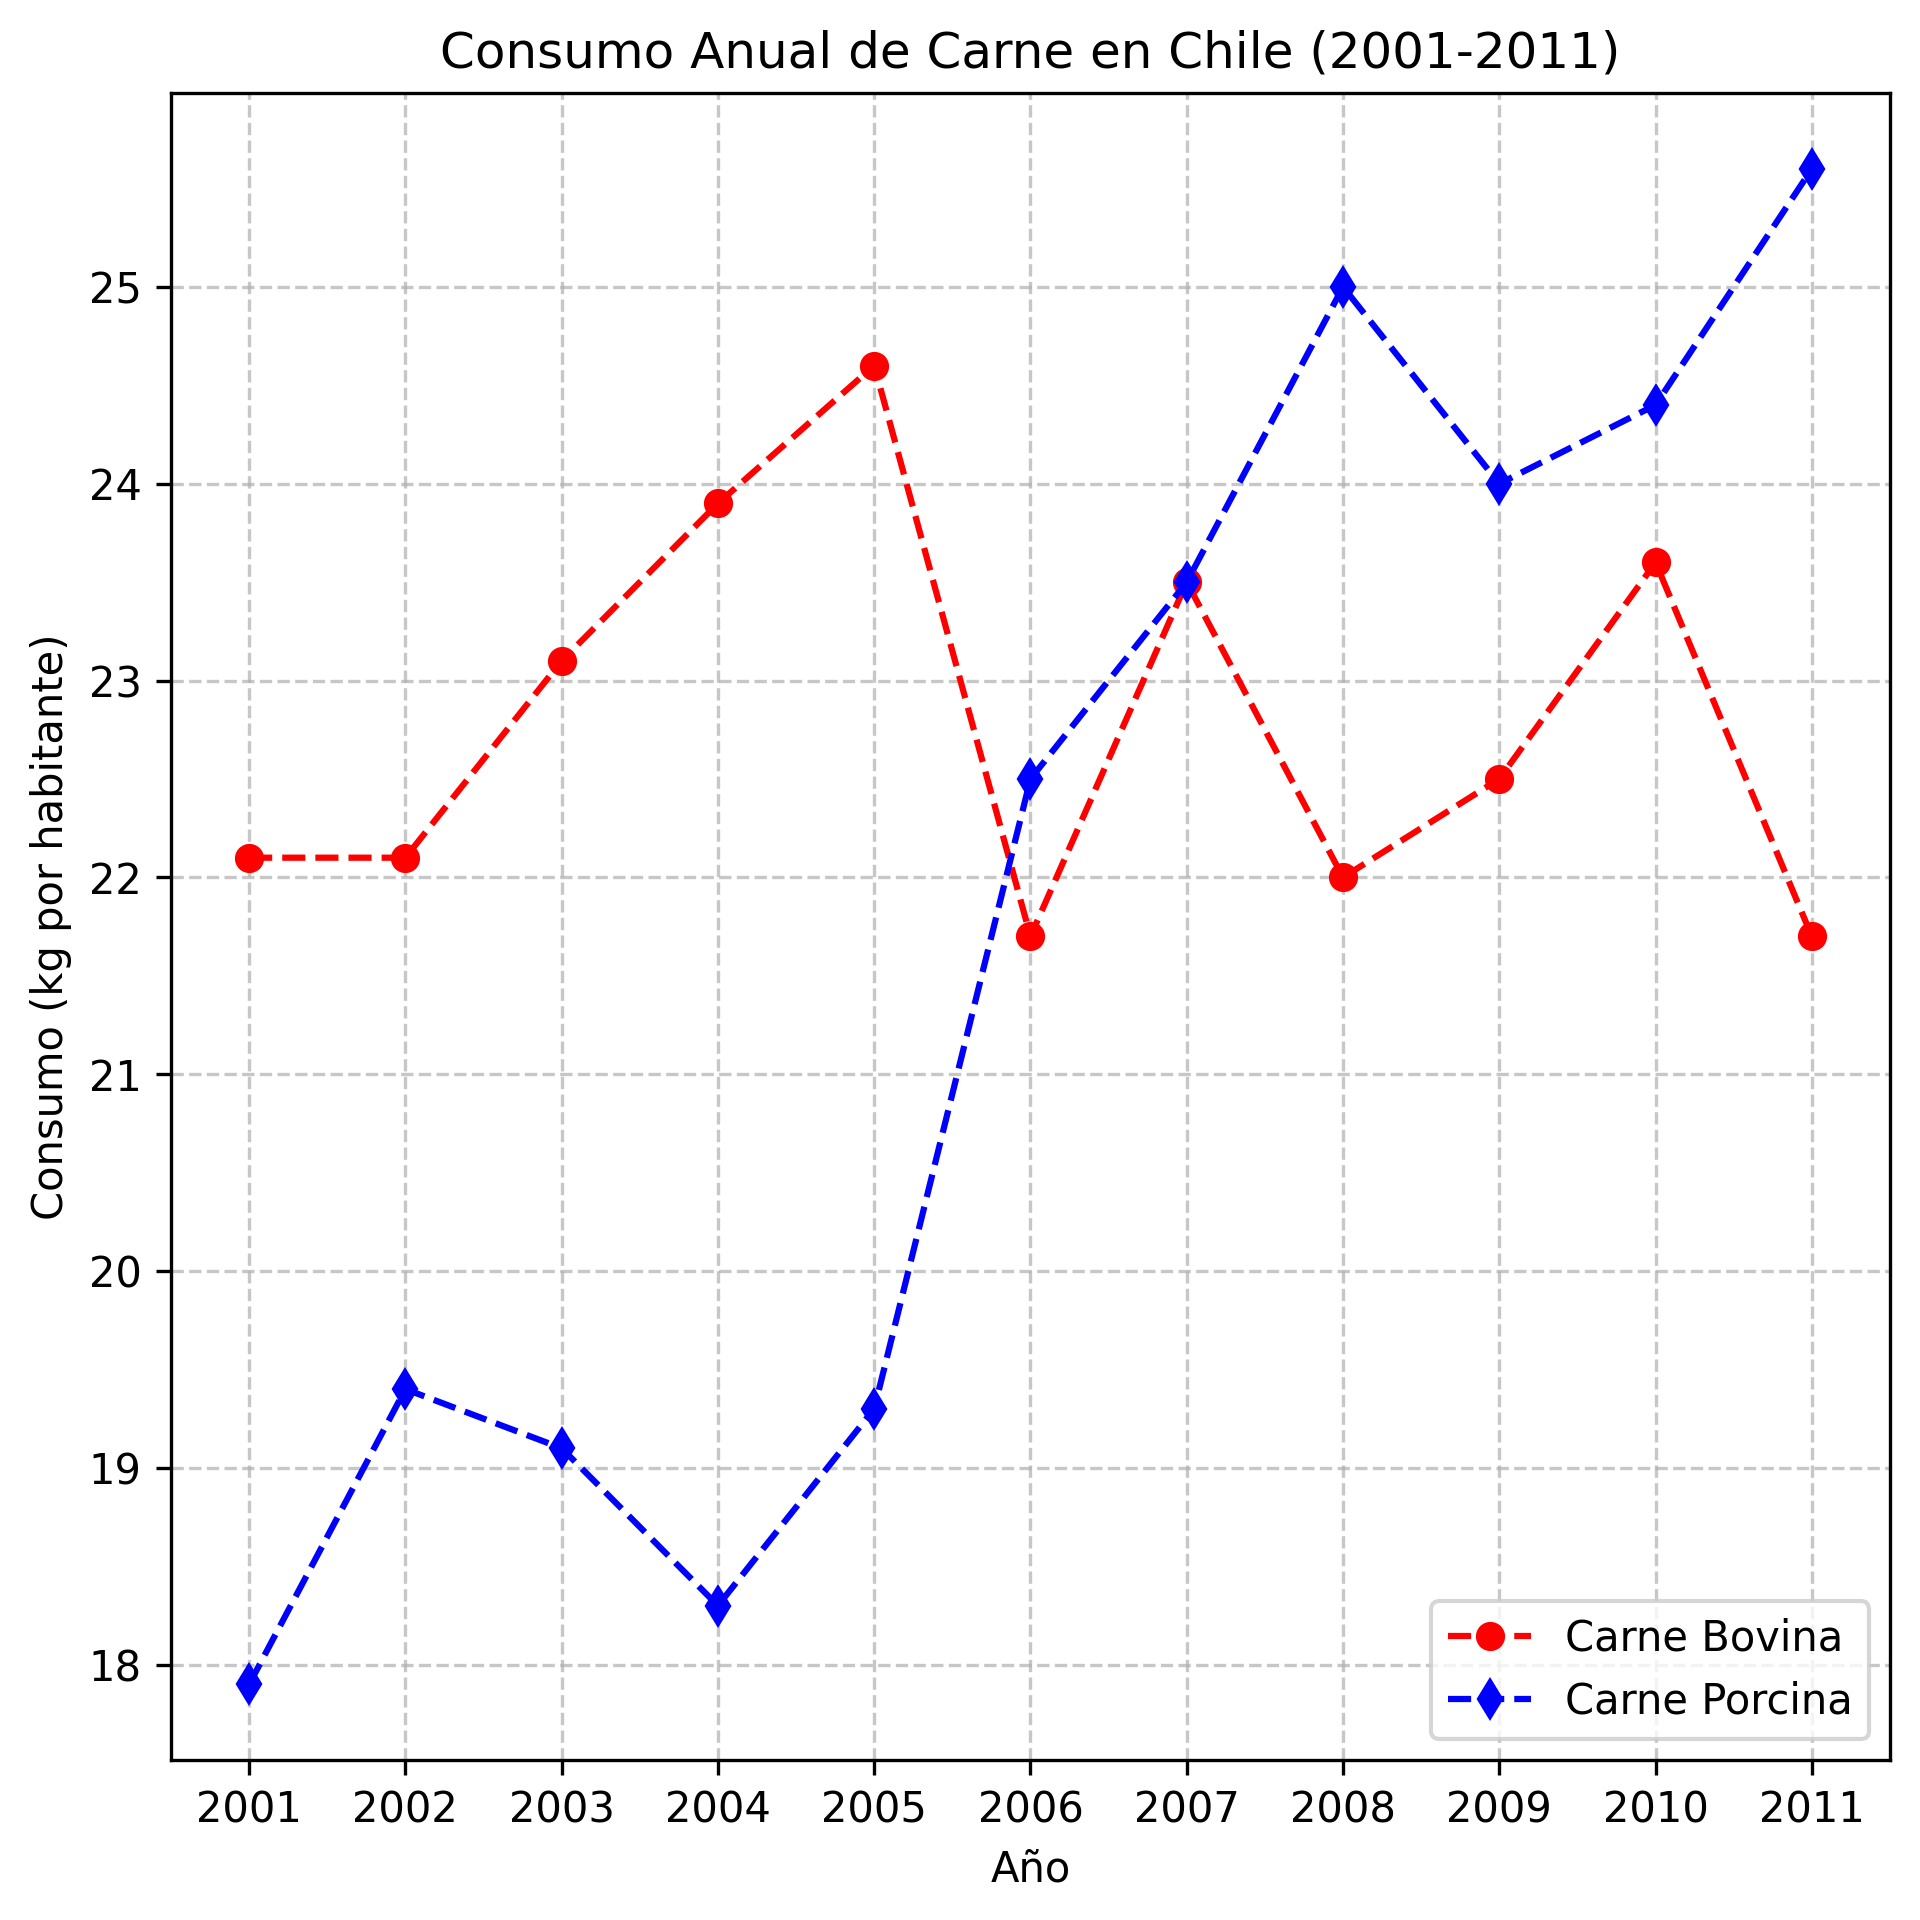
\includegraphics[keepaspectratio]{index_files/figure-pdf/cell-2-output-1.png}}

\pandocbounded{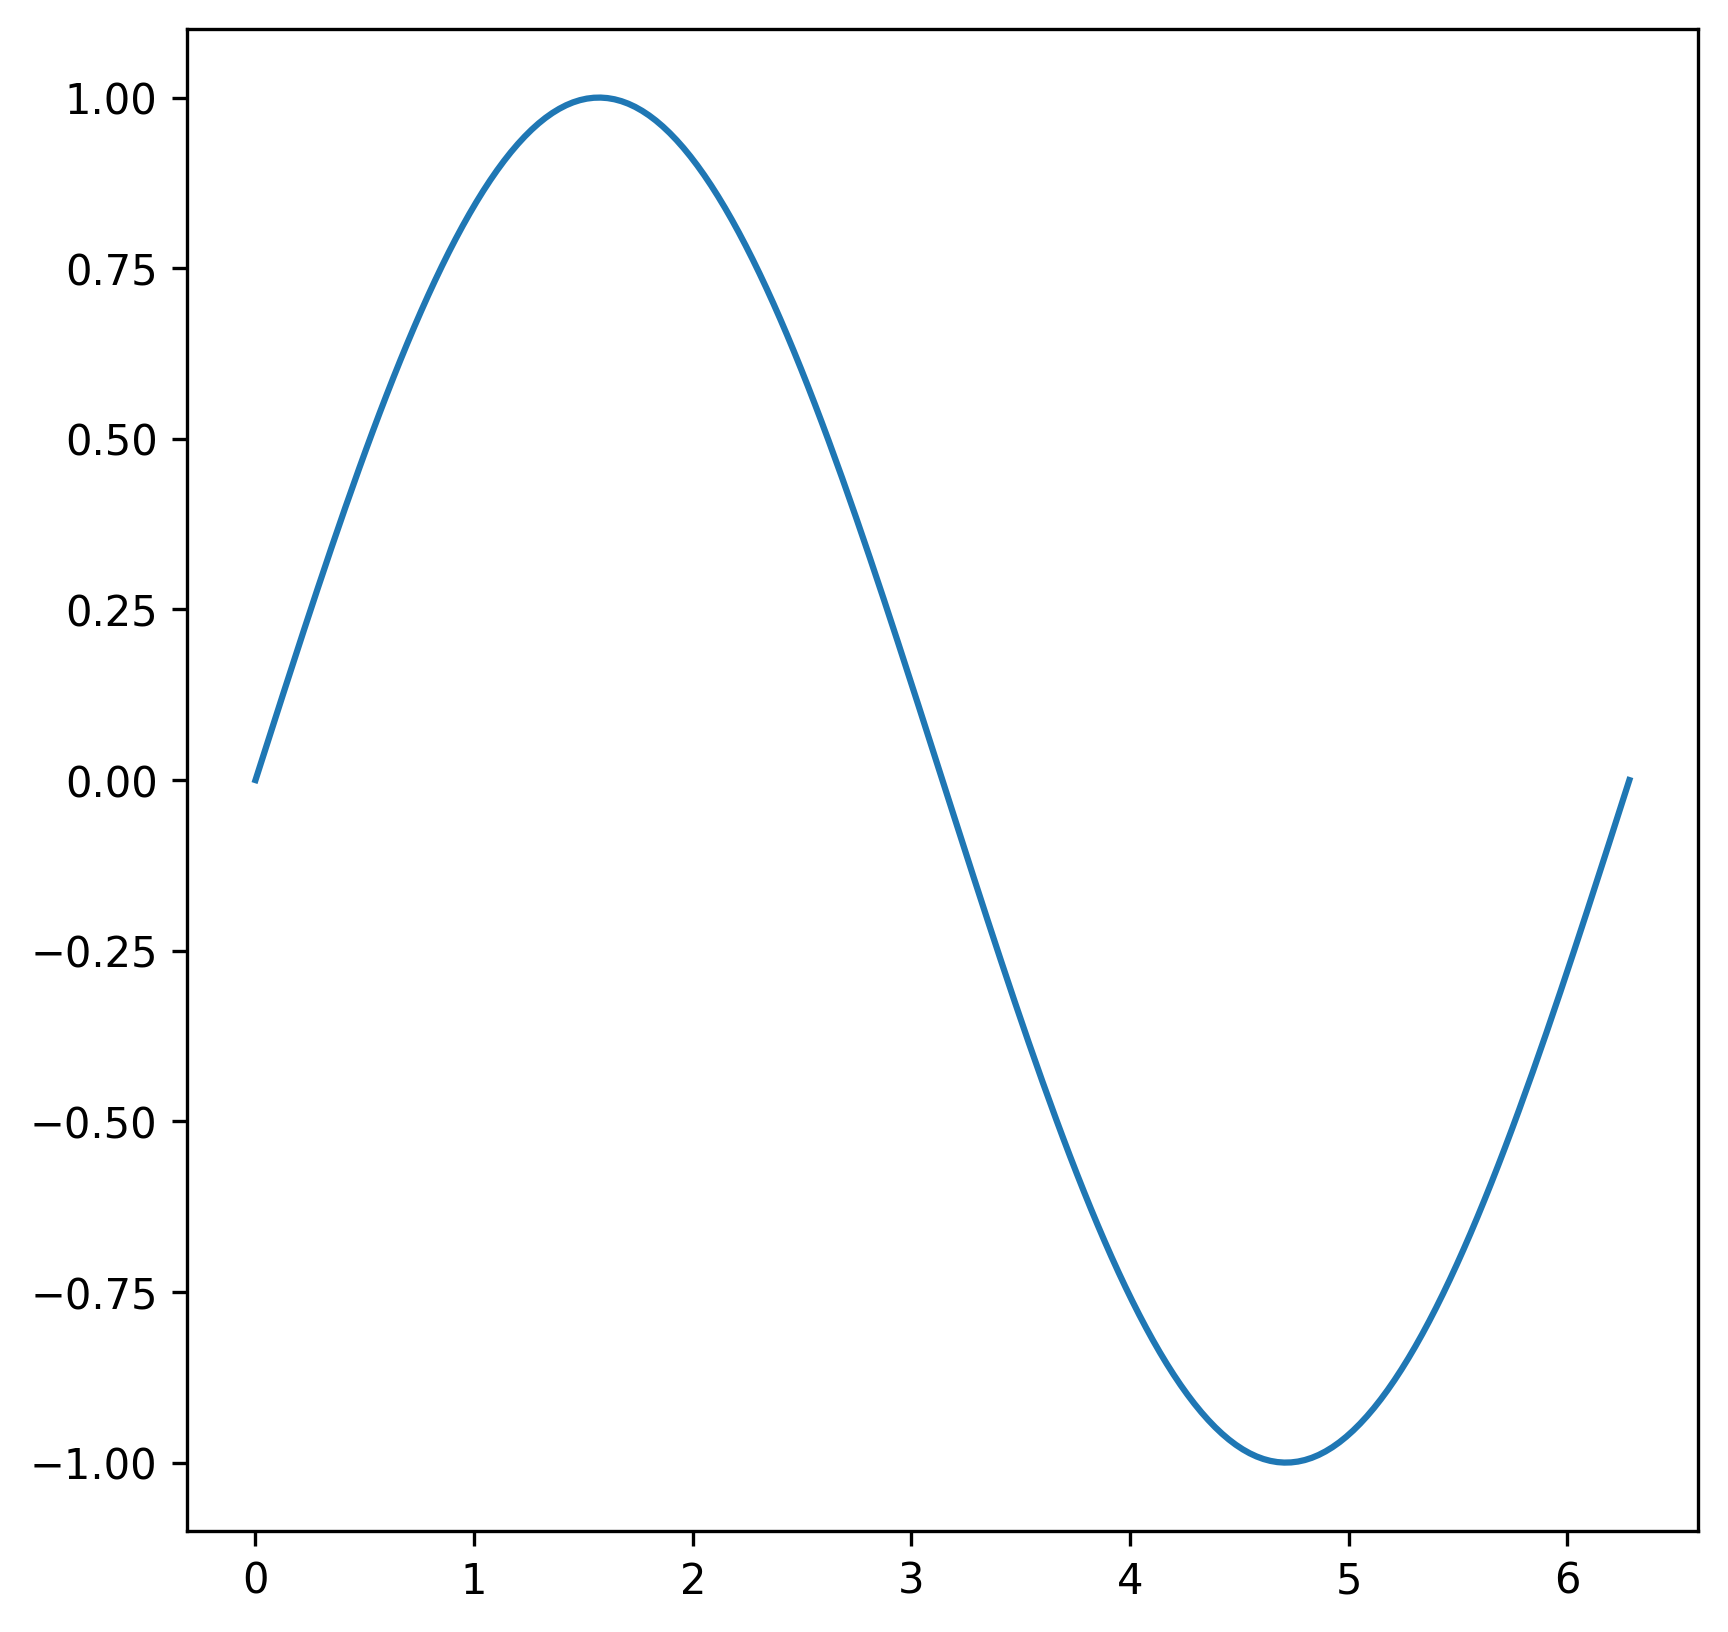
\includegraphics[keepaspectratio]{index_files/figure-pdf/cell-3-output-1.png}}

\begin{figure}

\caption{\label{fig-polar}A line plot on a polar axis}

\centering{

\pandocbounded{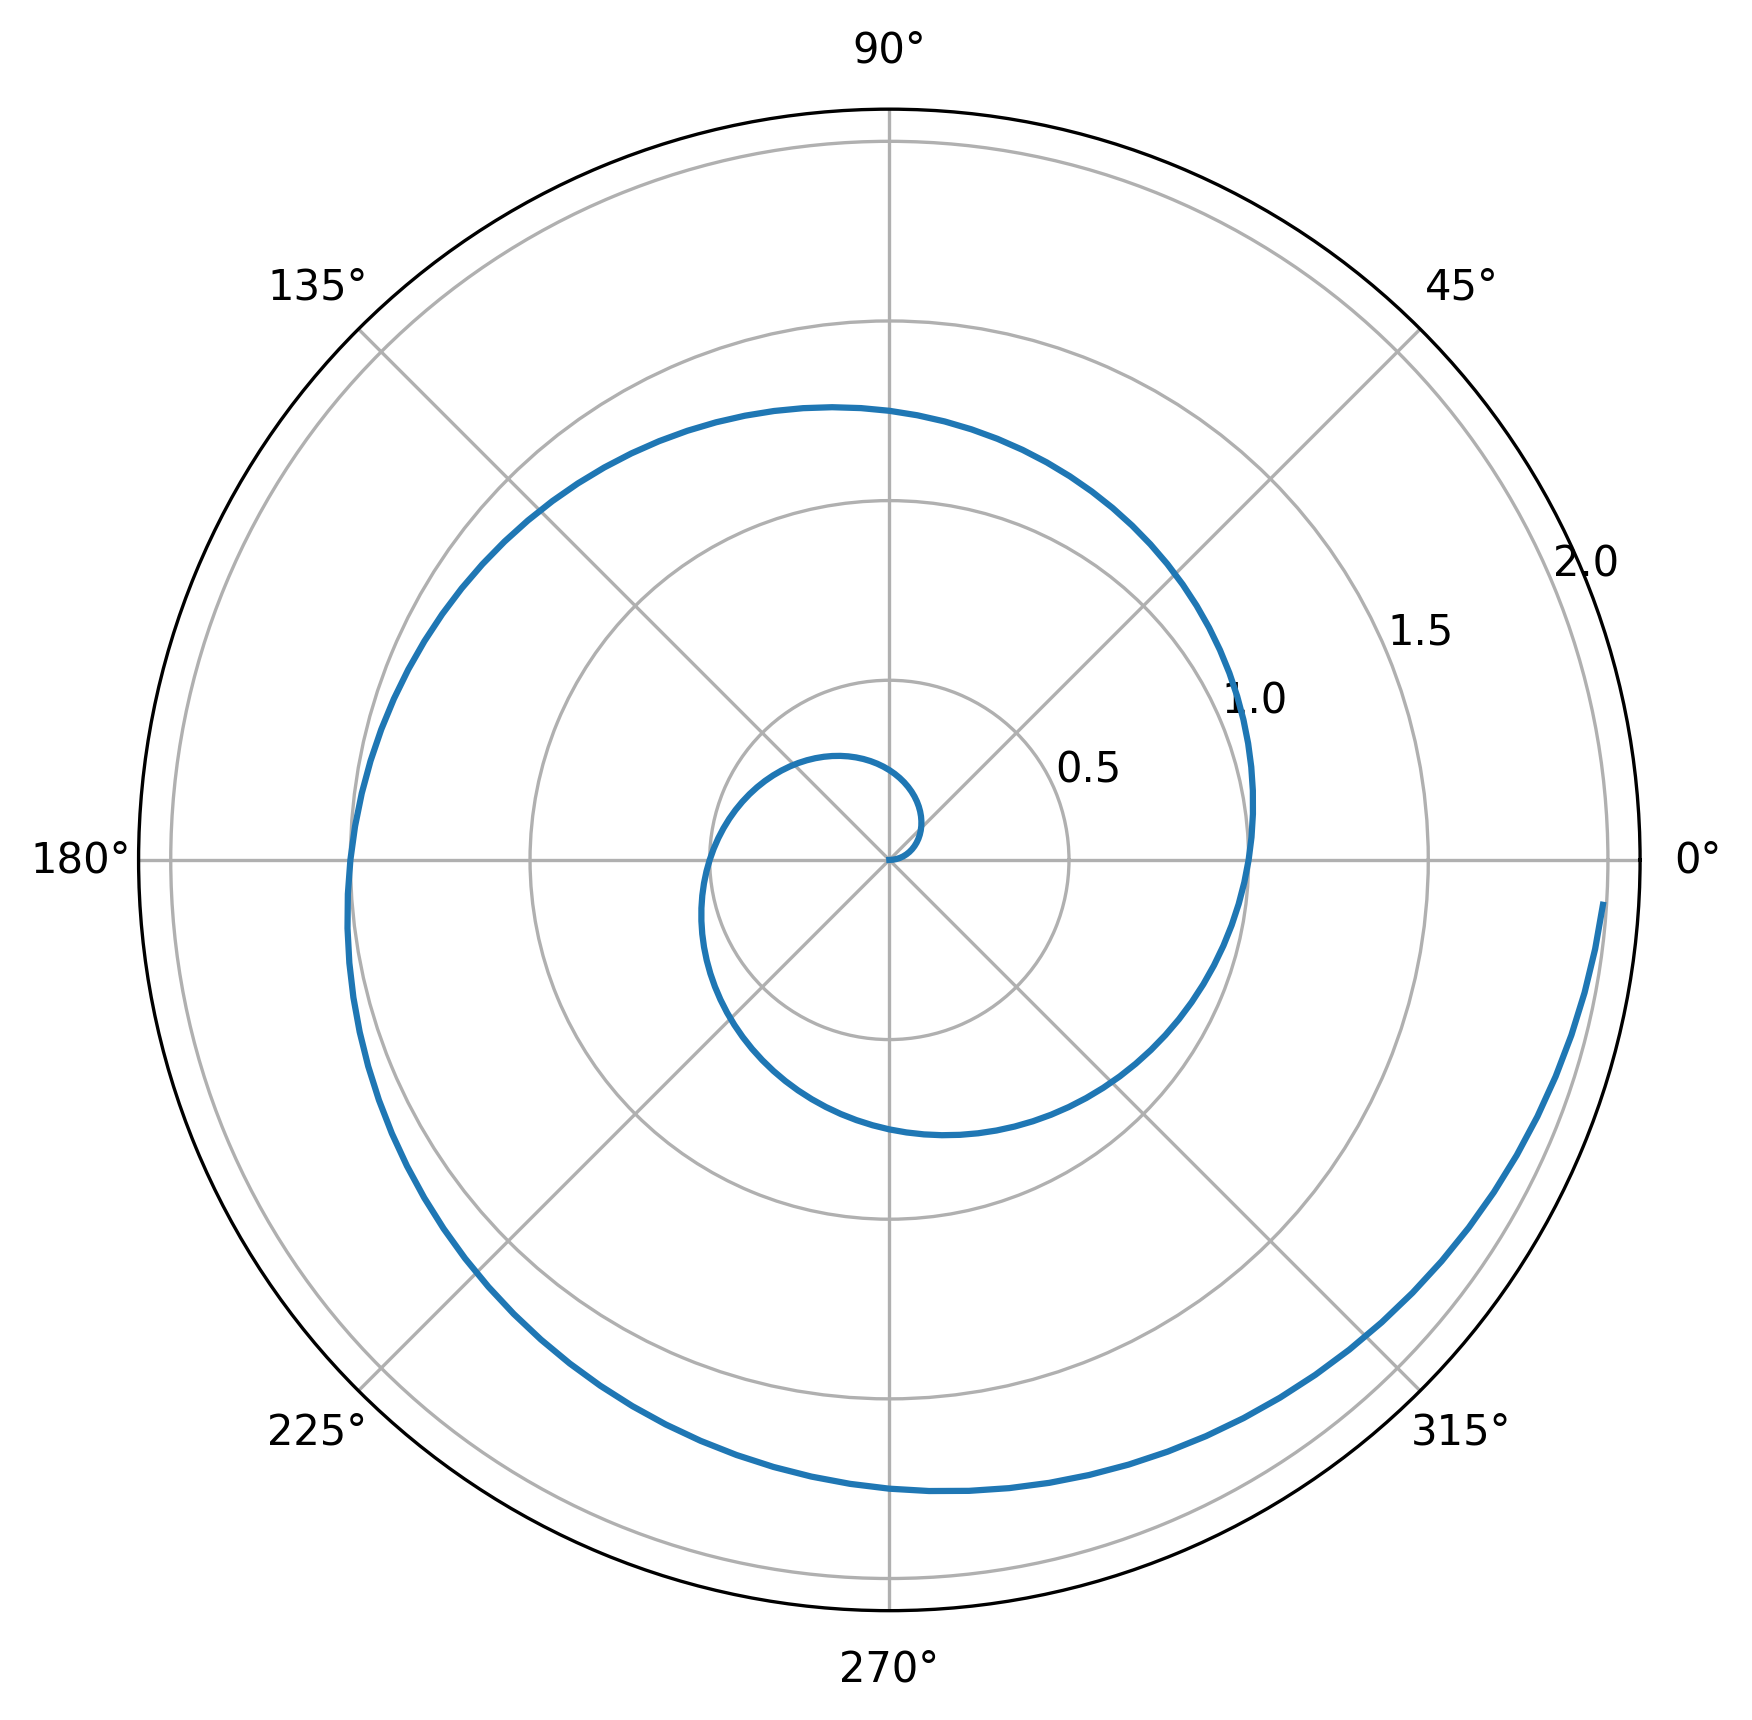
\includegraphics[keepaspectratio]{index_files/figure-pdf/fig-polar-output-1.png}}

}

\end{figure}%

\section{Gráfico de barras}\label{gruxe1fico-de-barras}

\subsection{horizontal}\label{horizontal}

\pandocbounded{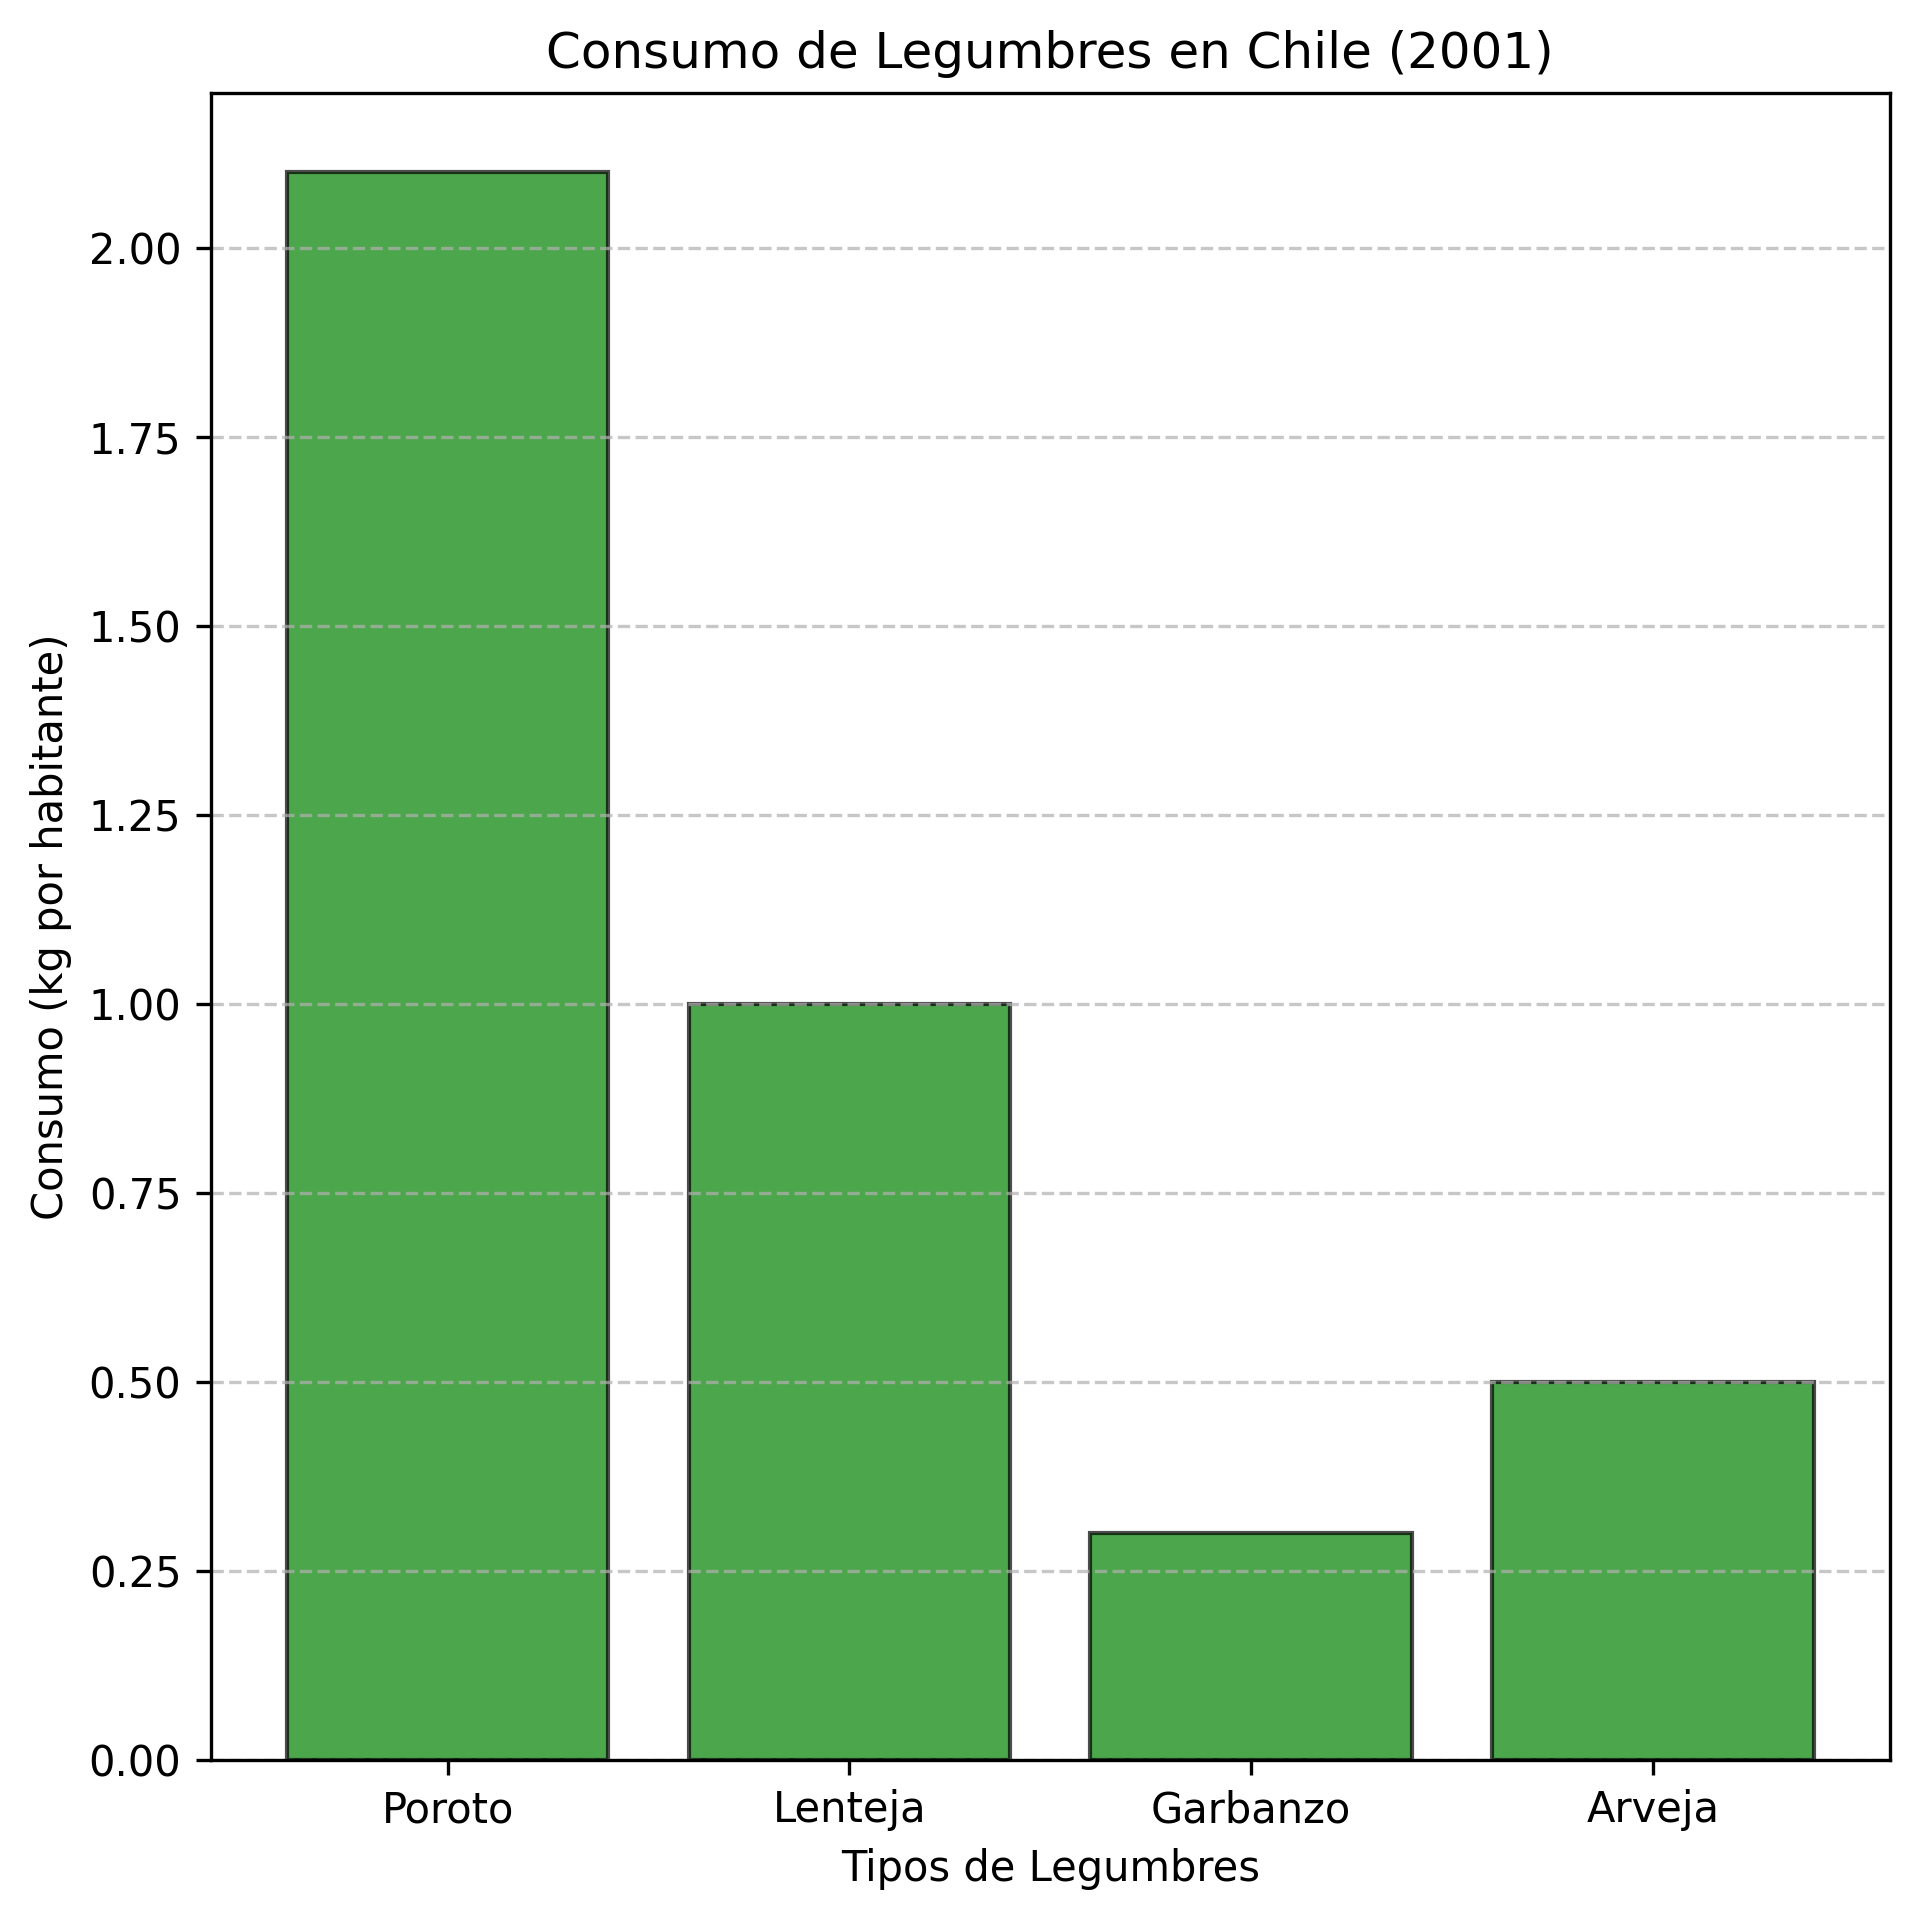
\includegraphics[keepaspectratio]{index_files/figure-pdf/cell-5-output-1.png}}

\subsection{vertical}\label{vertical}

\pandocbounded{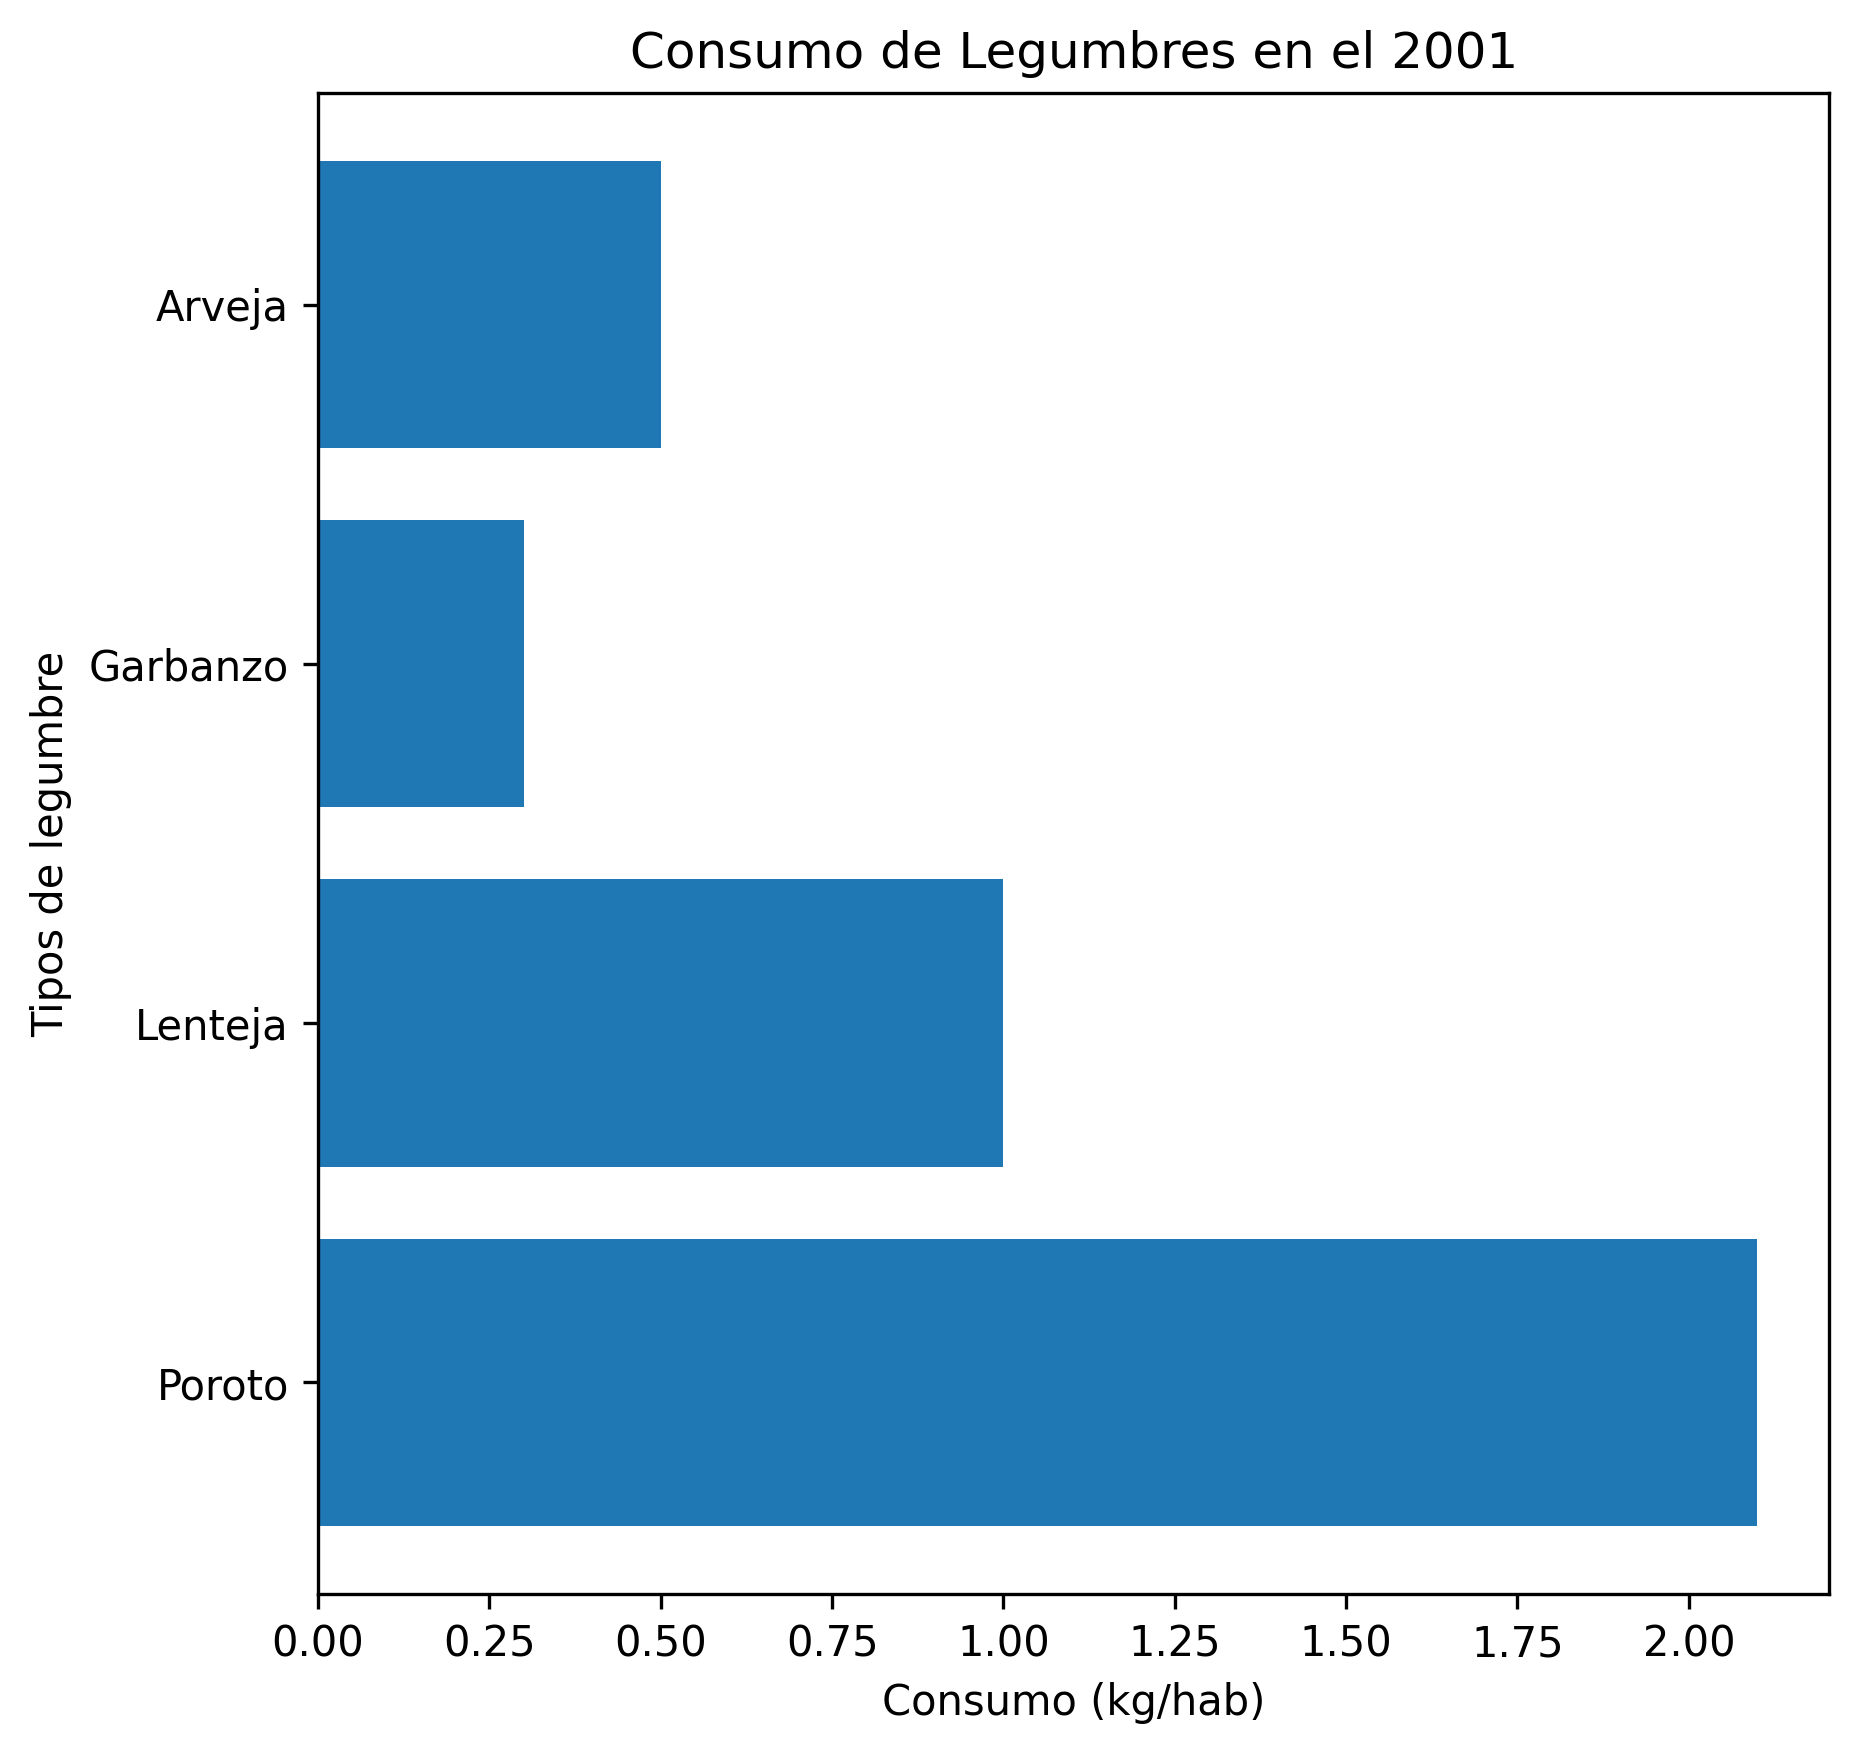
\includegraphics[keepaspectratio]{index_files/figure-pdf/cell-6-output-1.png}}

\section{Histograma}\label{histograma}

\pandocbounded{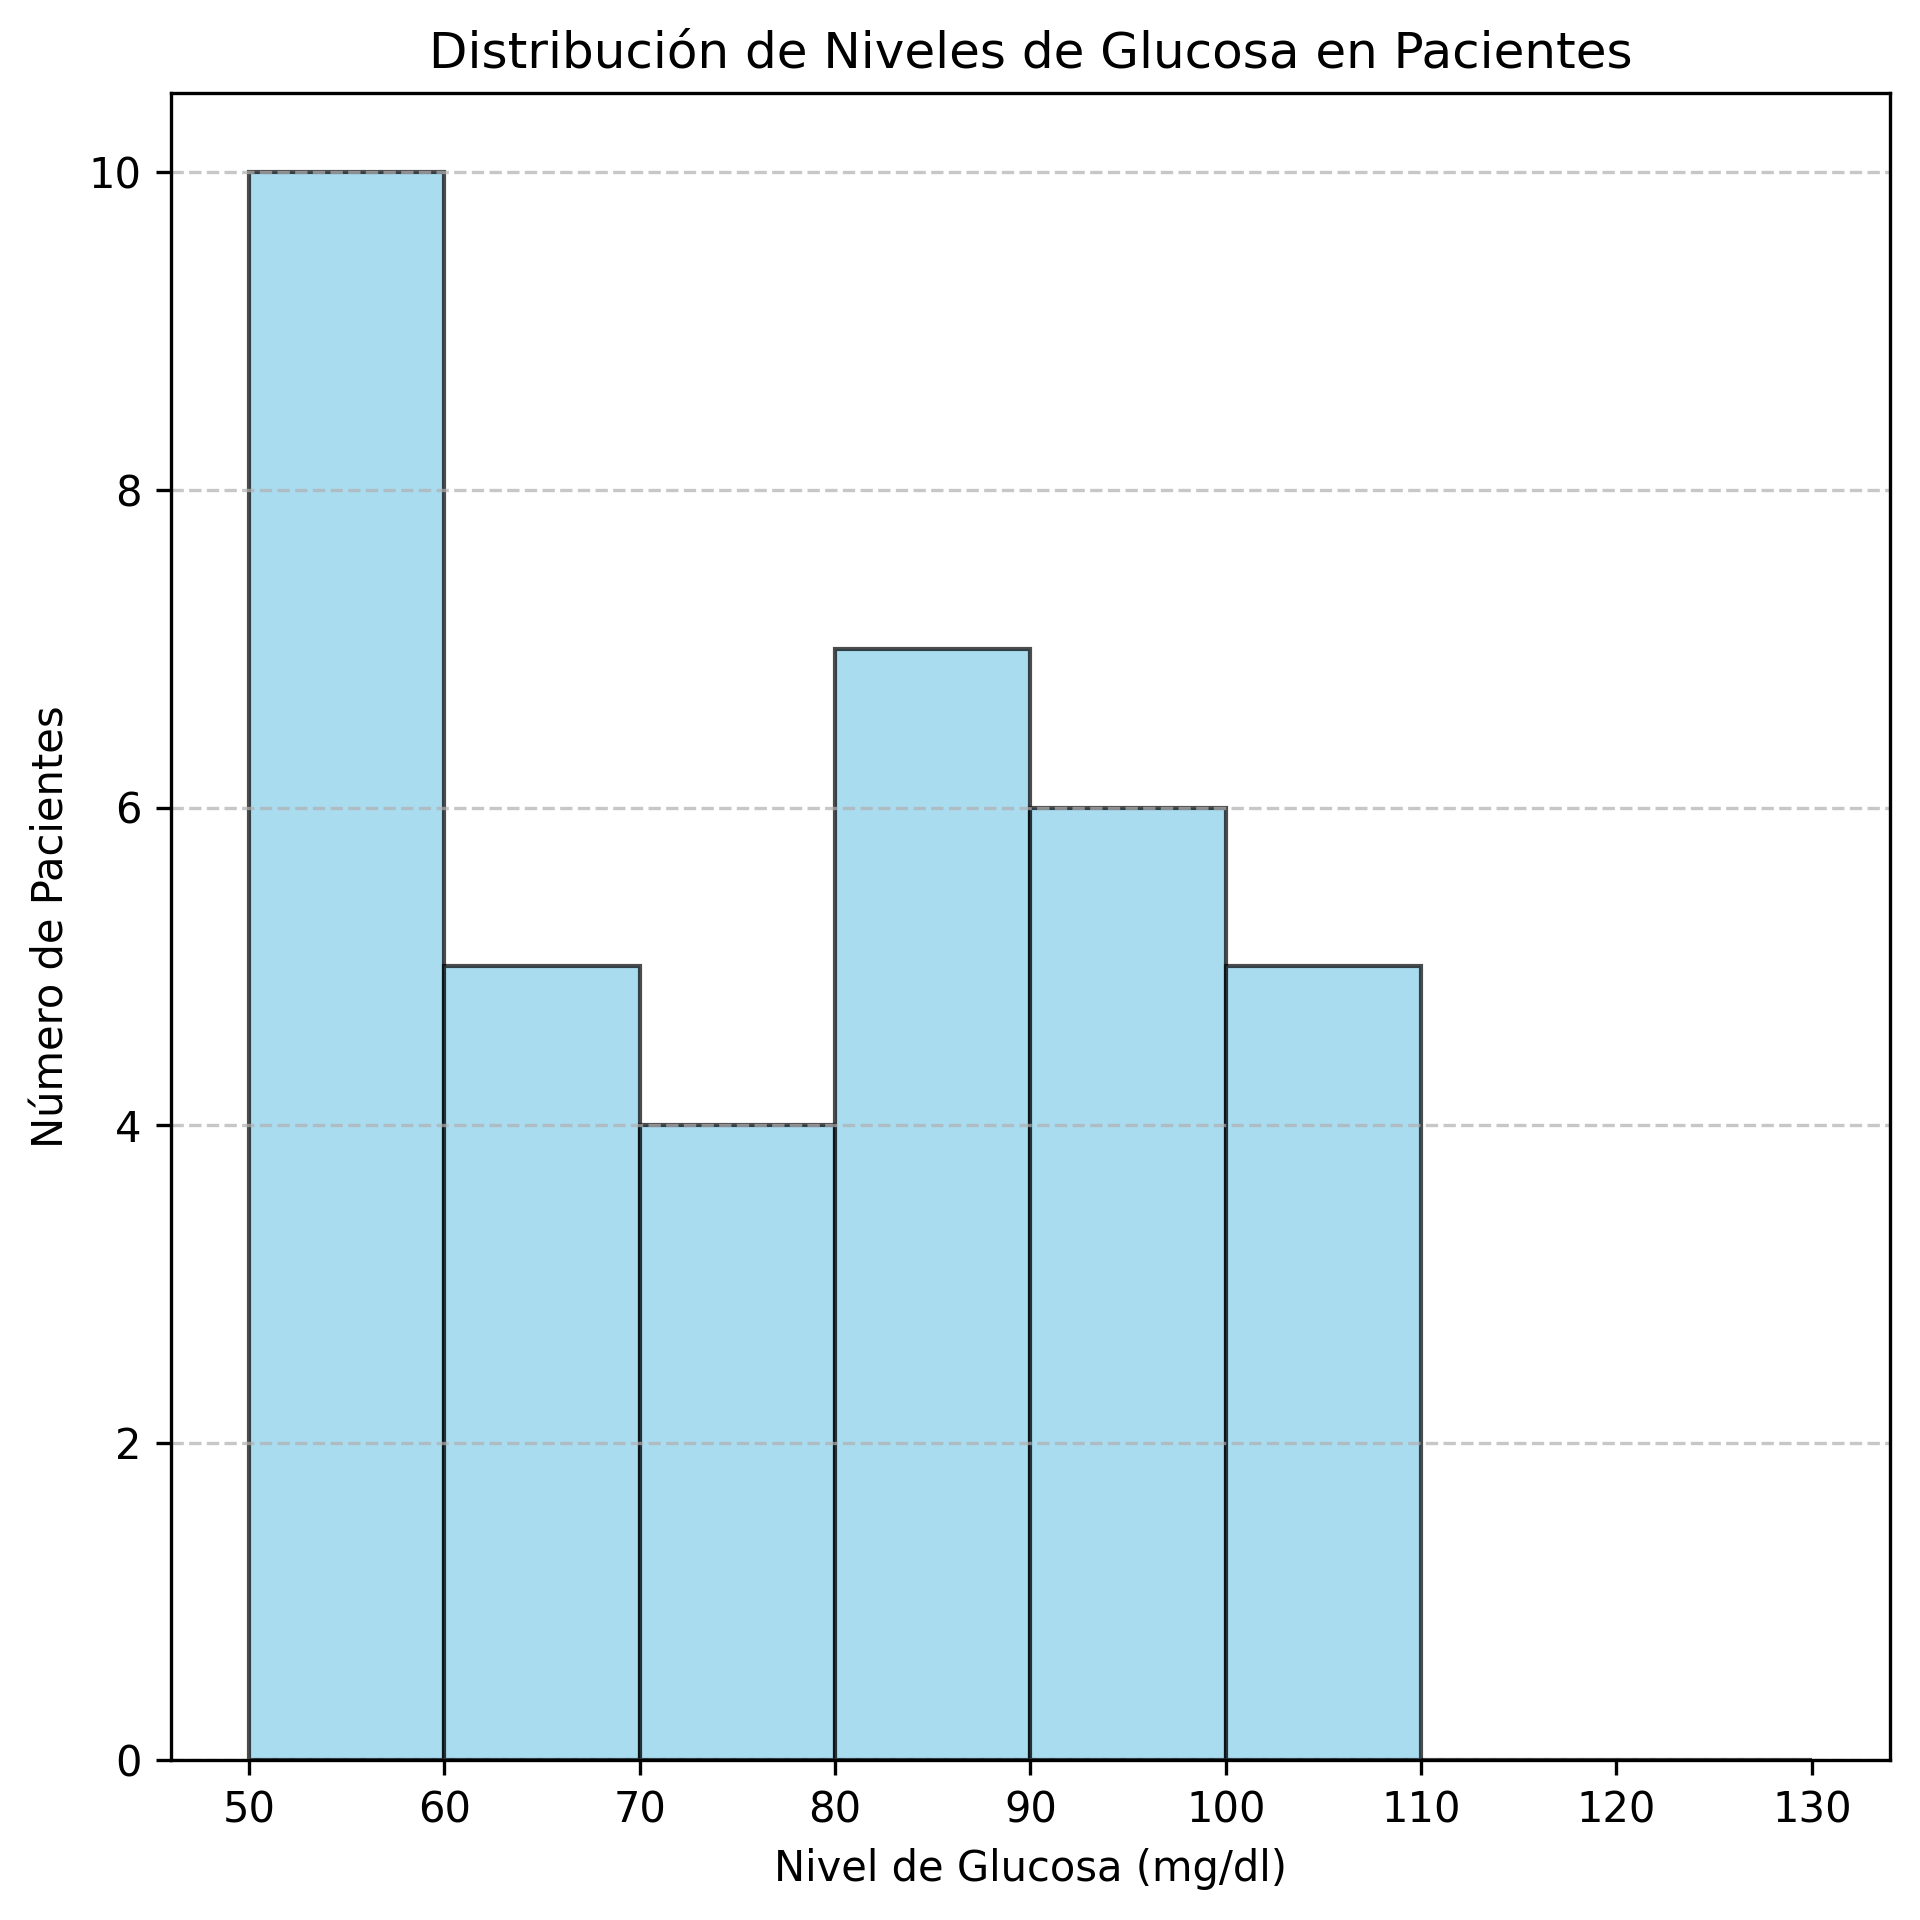
\includegraphics[keepaspectratio]{index_files/figure-pdf/cell-7-output-1.png}}

\section{Grafico circular}\label{grafico-circular}

\pandocbounded{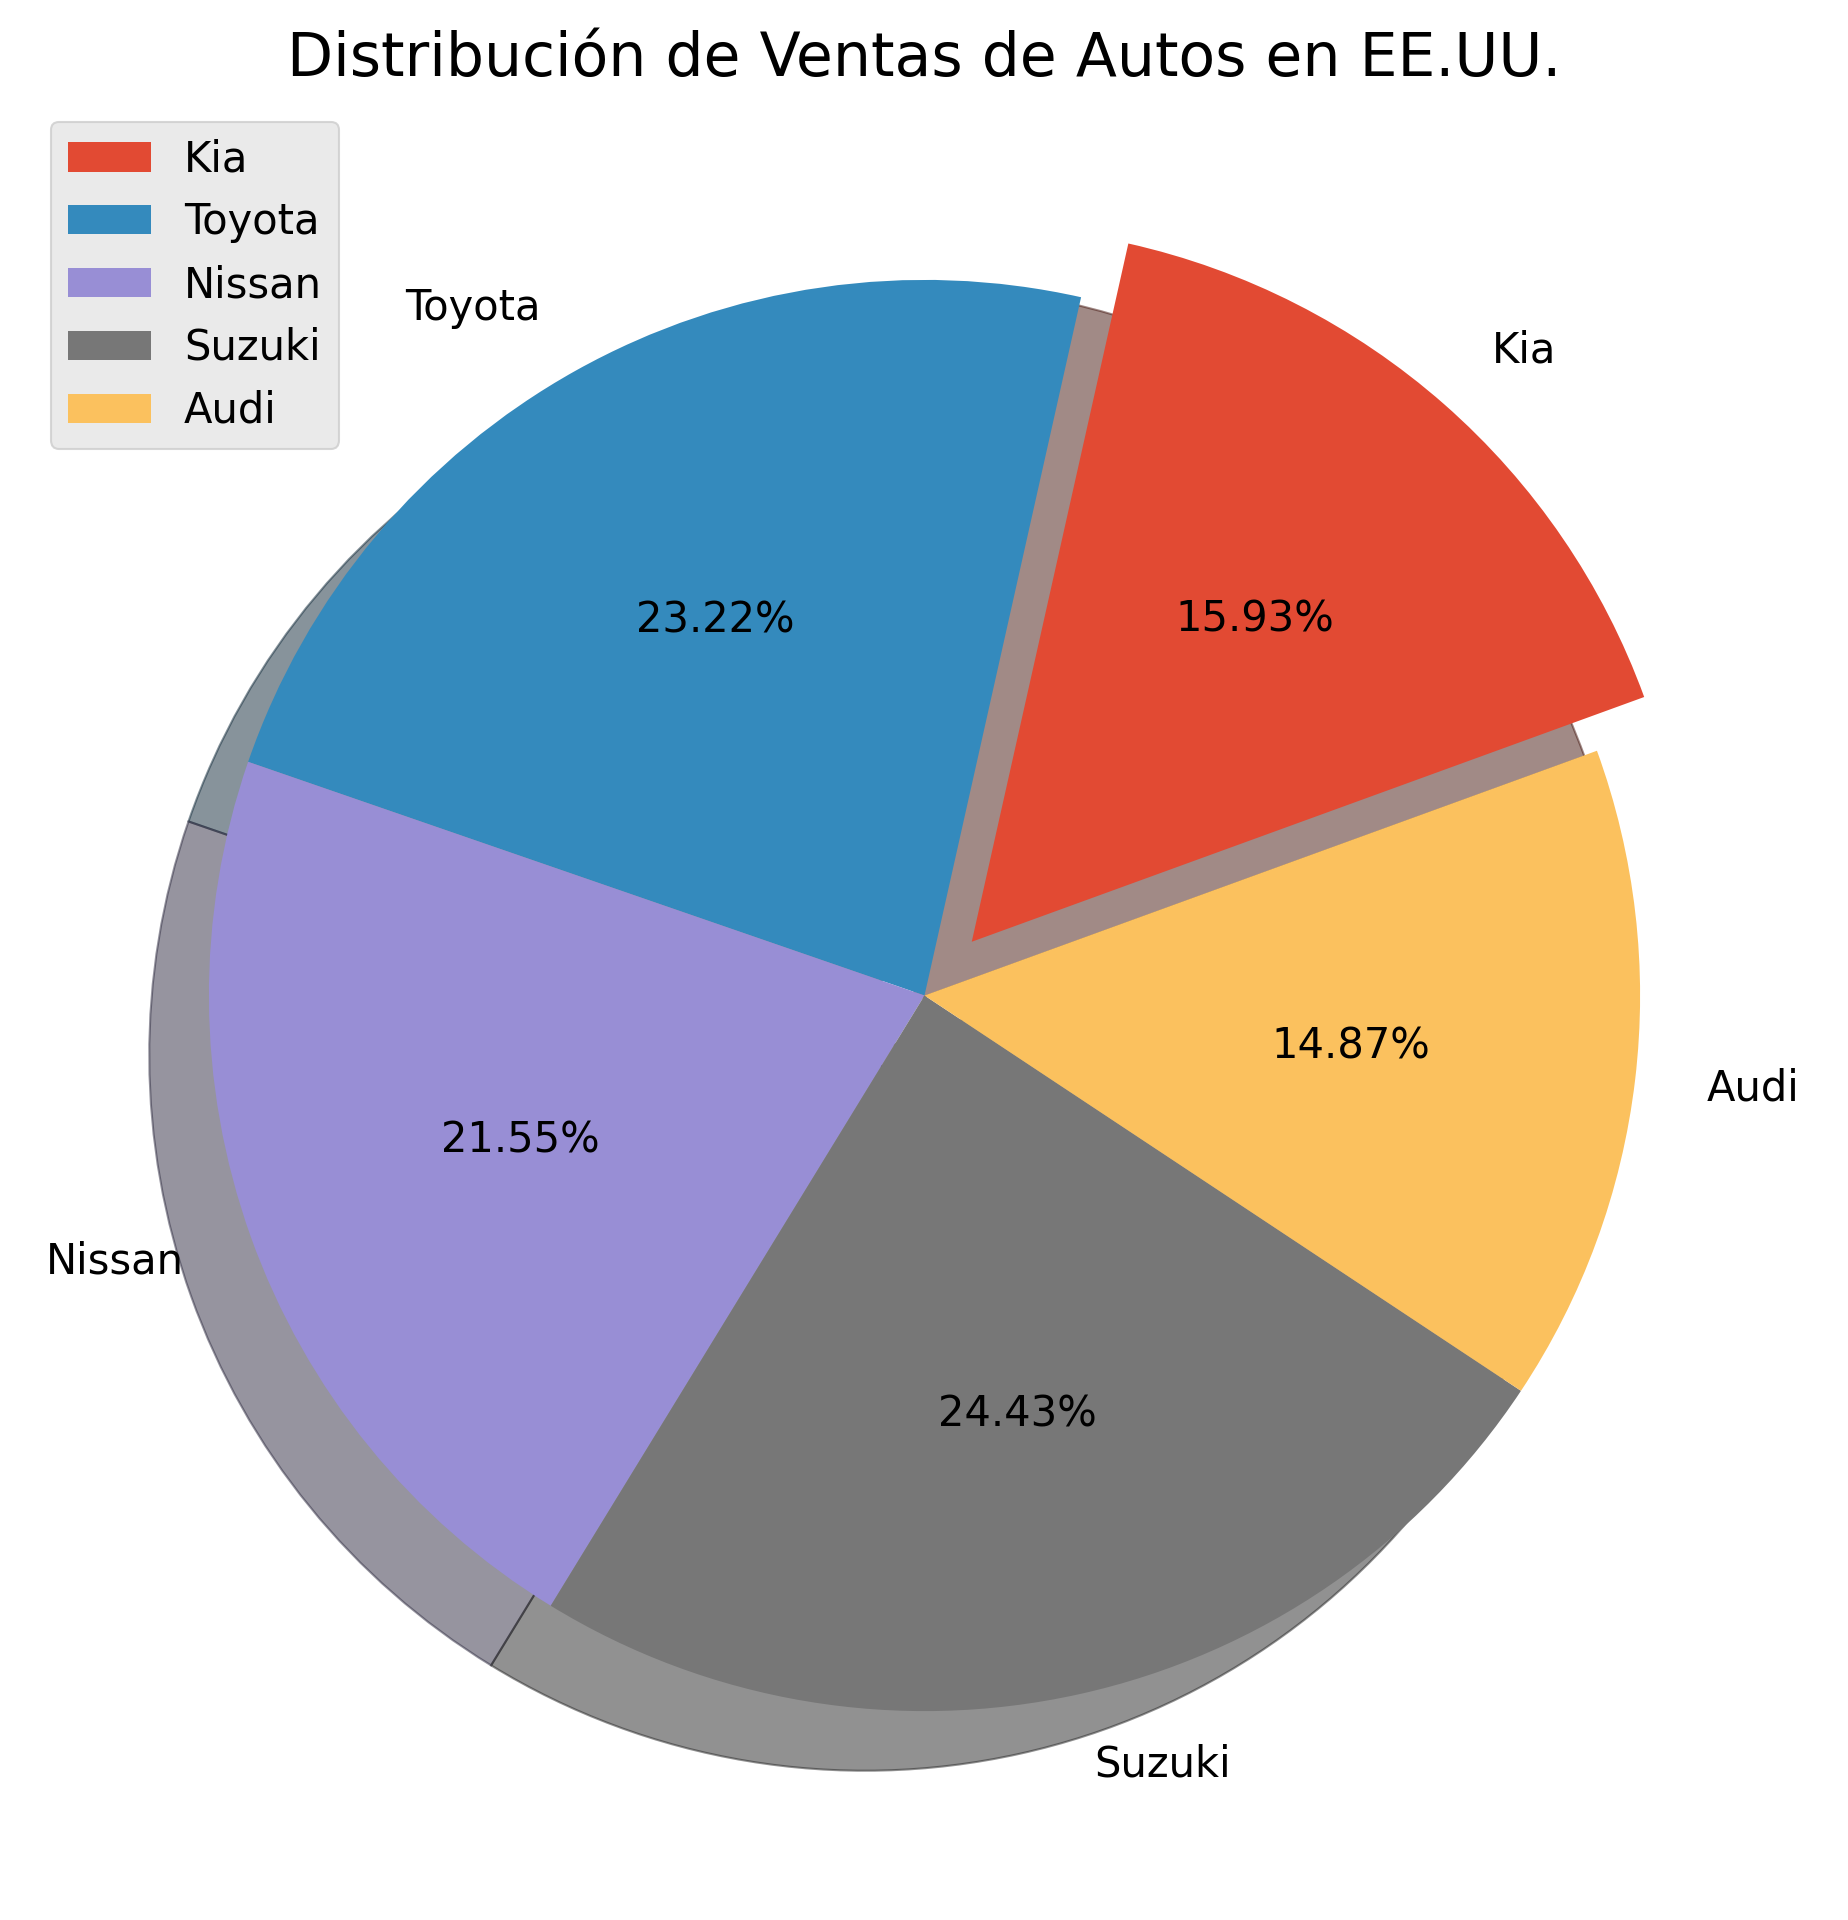
\includegraphics[keepaspectratio]{index_files/figure-pdf/cell-8-output-1.png}}

\section{Grafico de Donut}\label{grafico-de-donut}

\pandocbounded{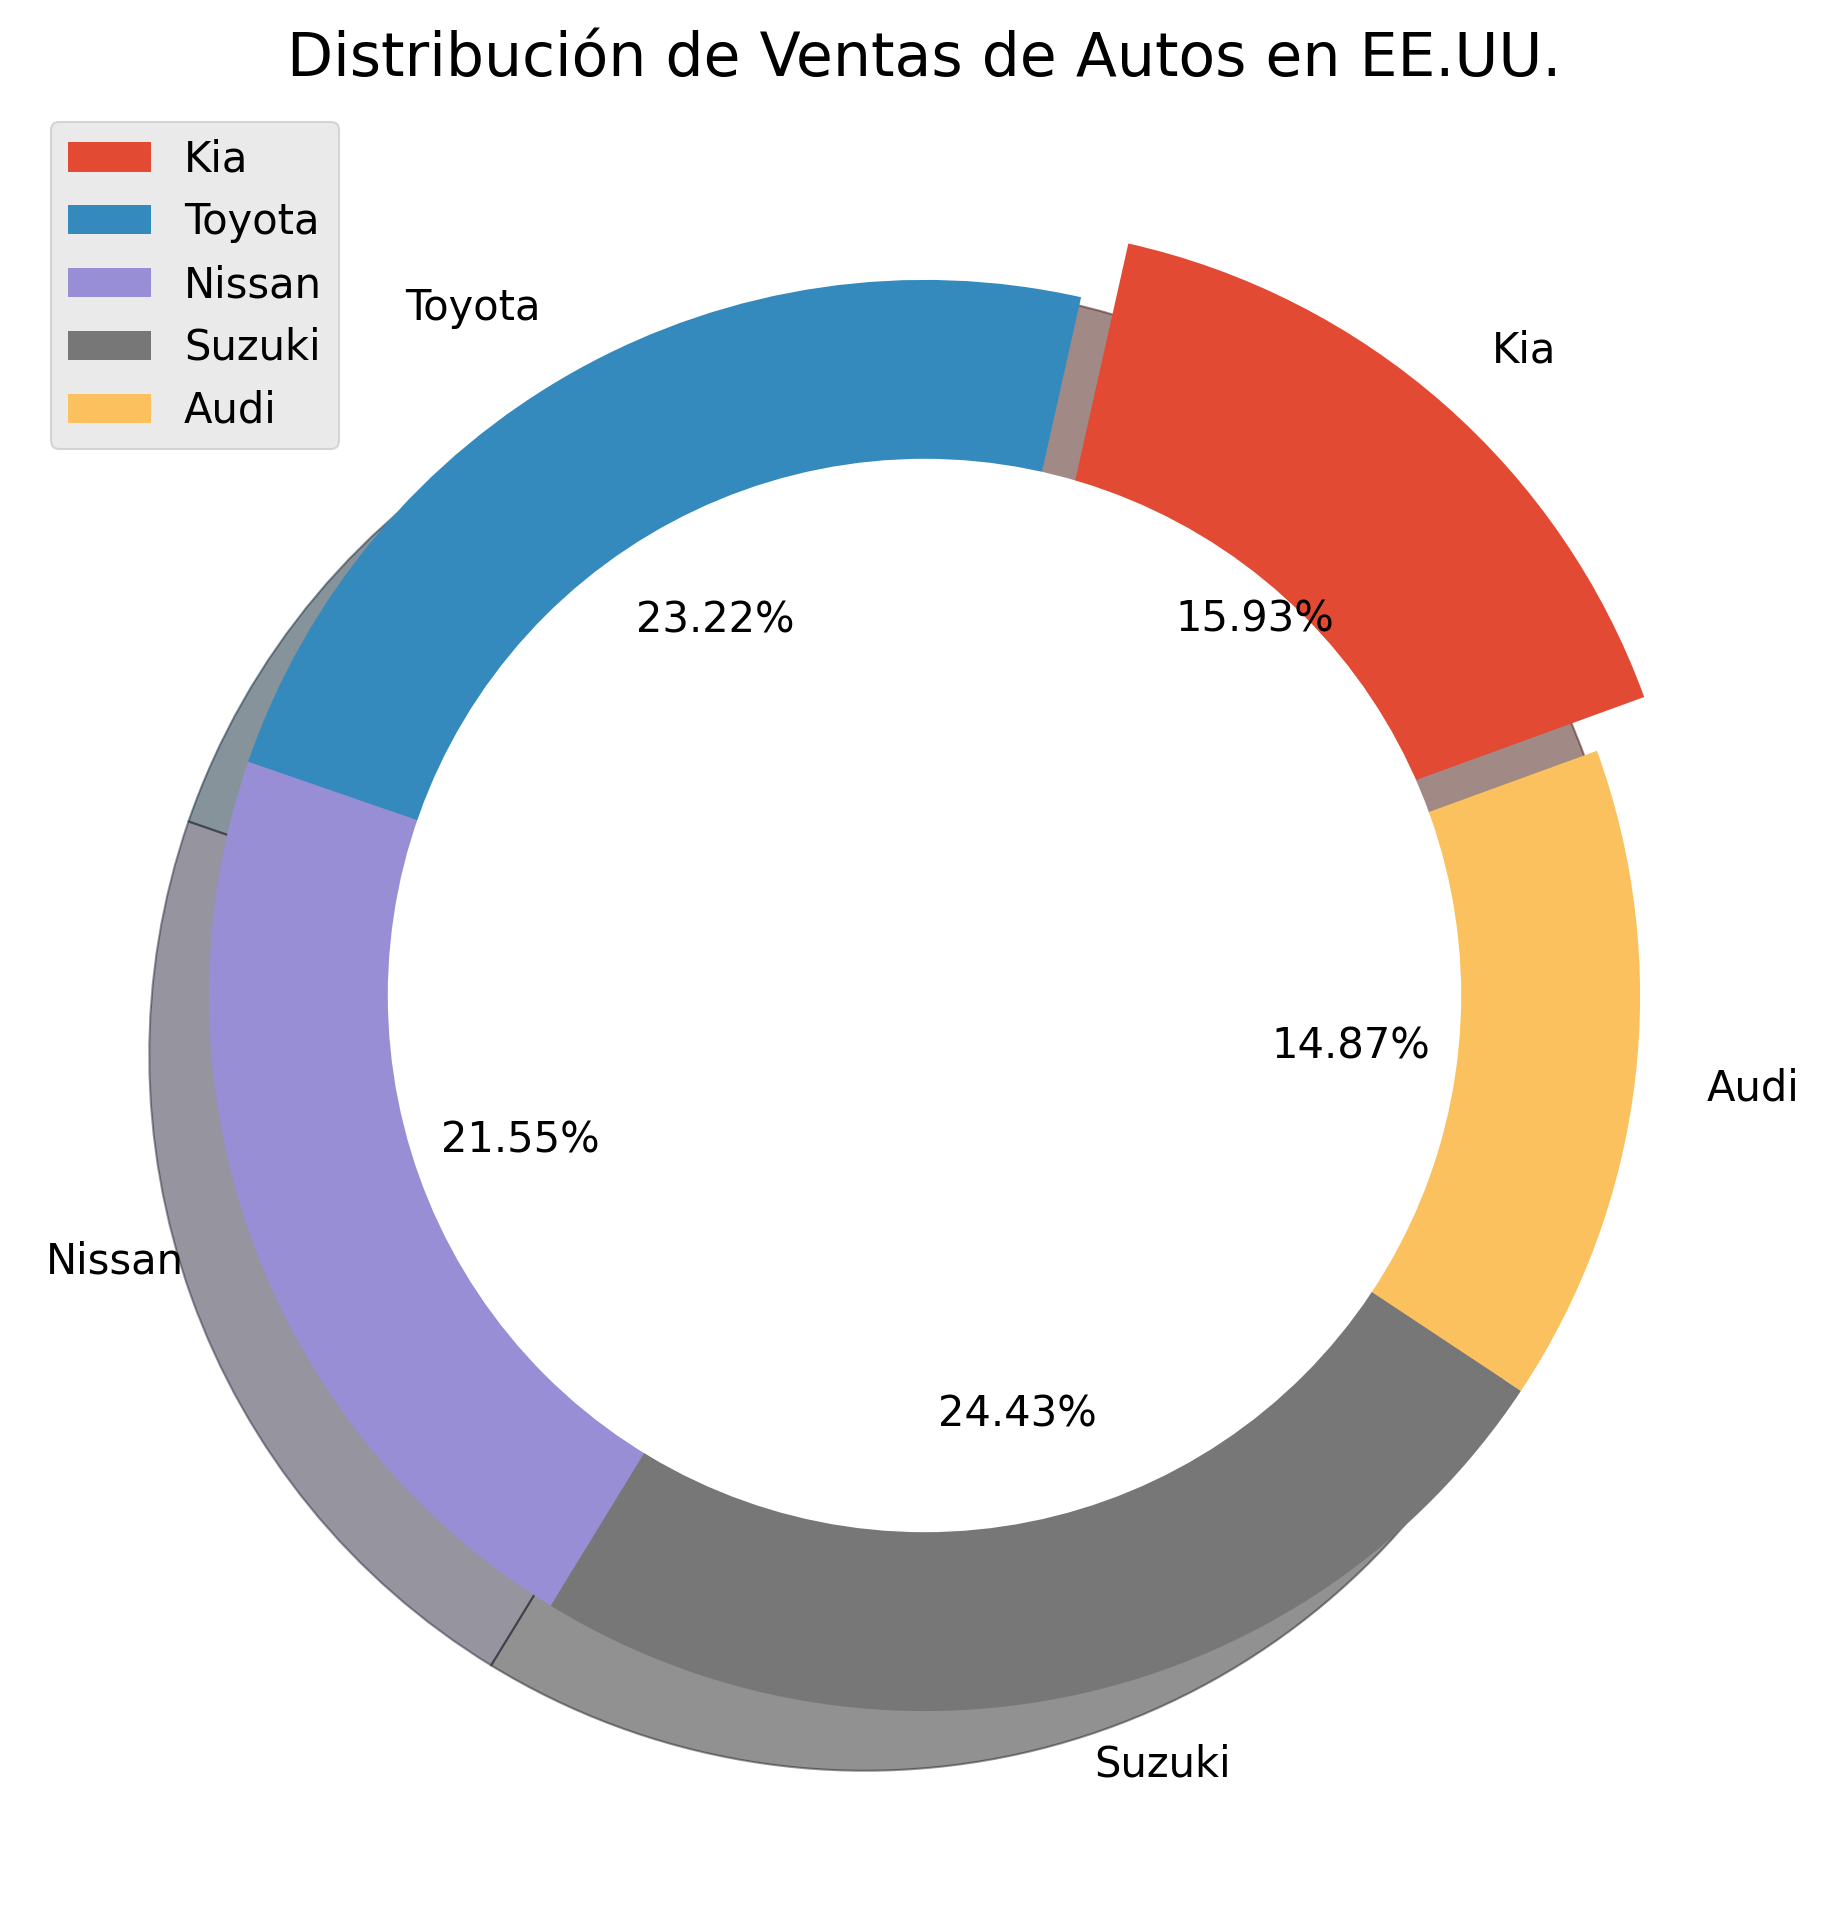
\includegraphics[keepaspectratio]{index_files/figure-pdf/cell-9-output-1.png}}

\section{Grafico de cajas}\label{grafico-de-cajas}

\pandocbounded{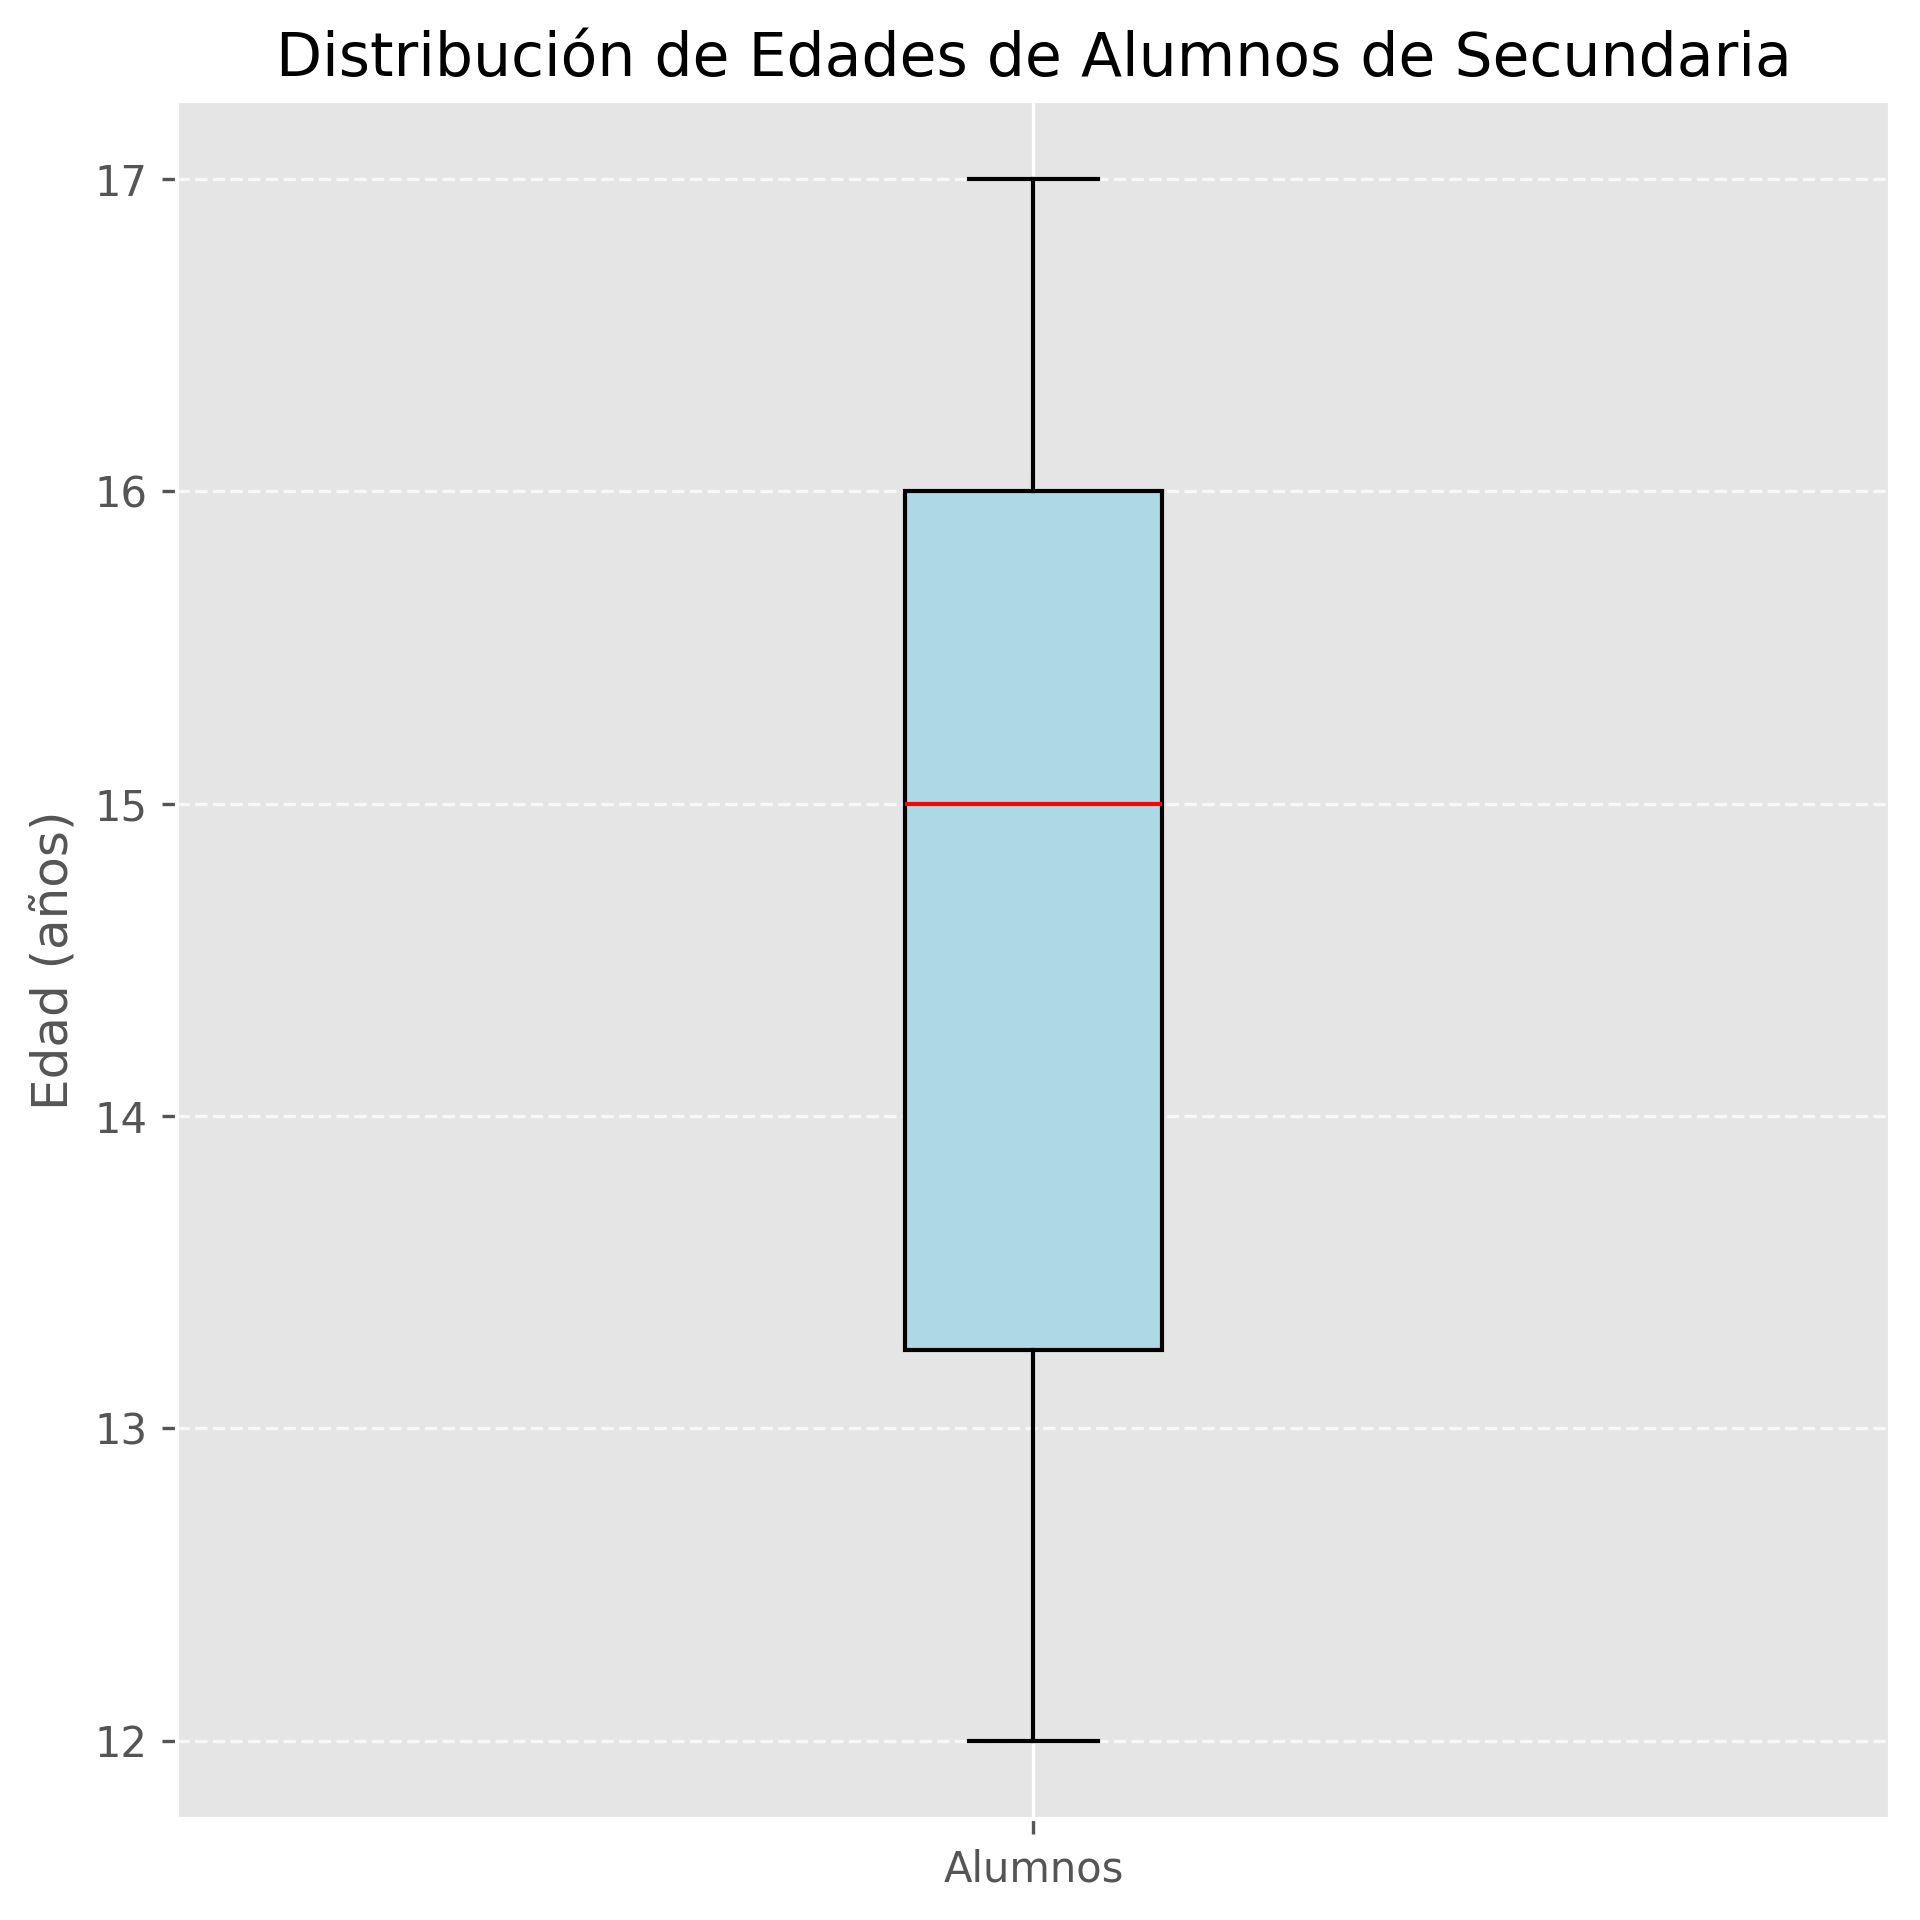
\includegraphics[keepaspectratio]{index_files/figure-pdf/cell-10-output-1.png}}

\section{Grafico de barras
combinadas}\label{grafico-de-barras-combinadas}

\pandocbounded{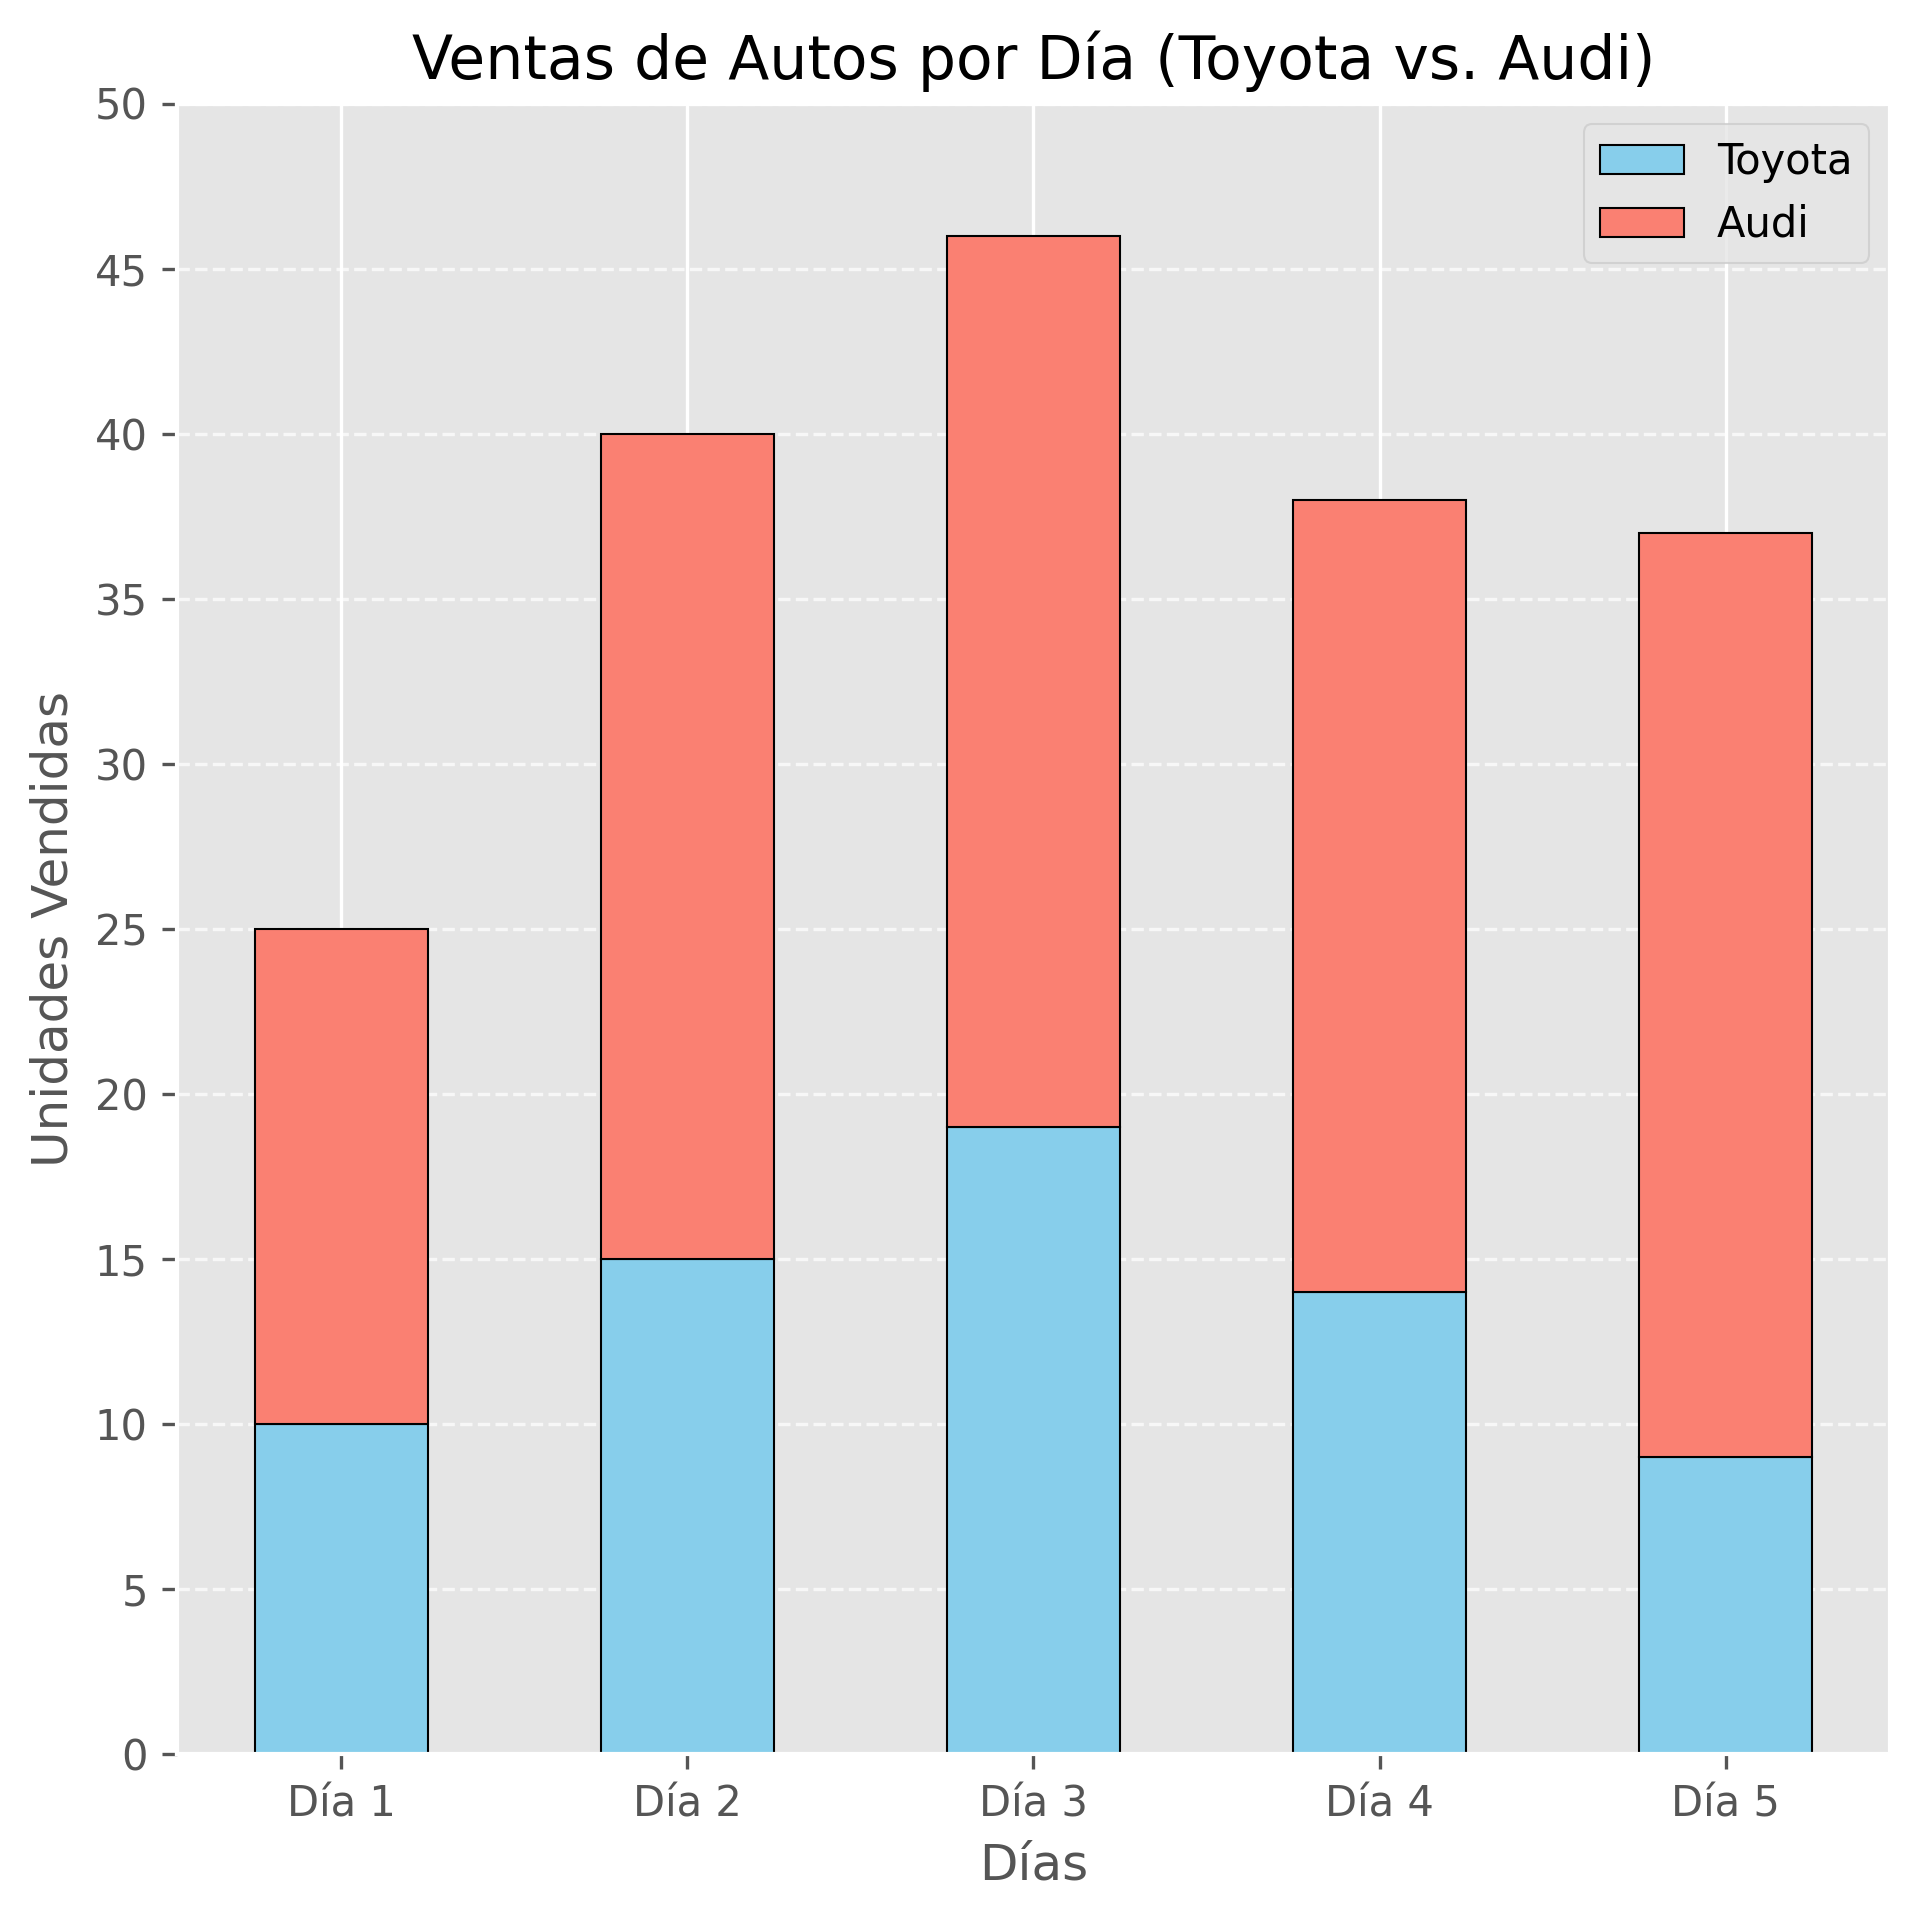
\includegraphics[keepaspectratio]{index_files/figure-pdf/cell-11-output-1.png}}

\section{Graficos combinados}\label{graficos-combinados}

\pandocbounded{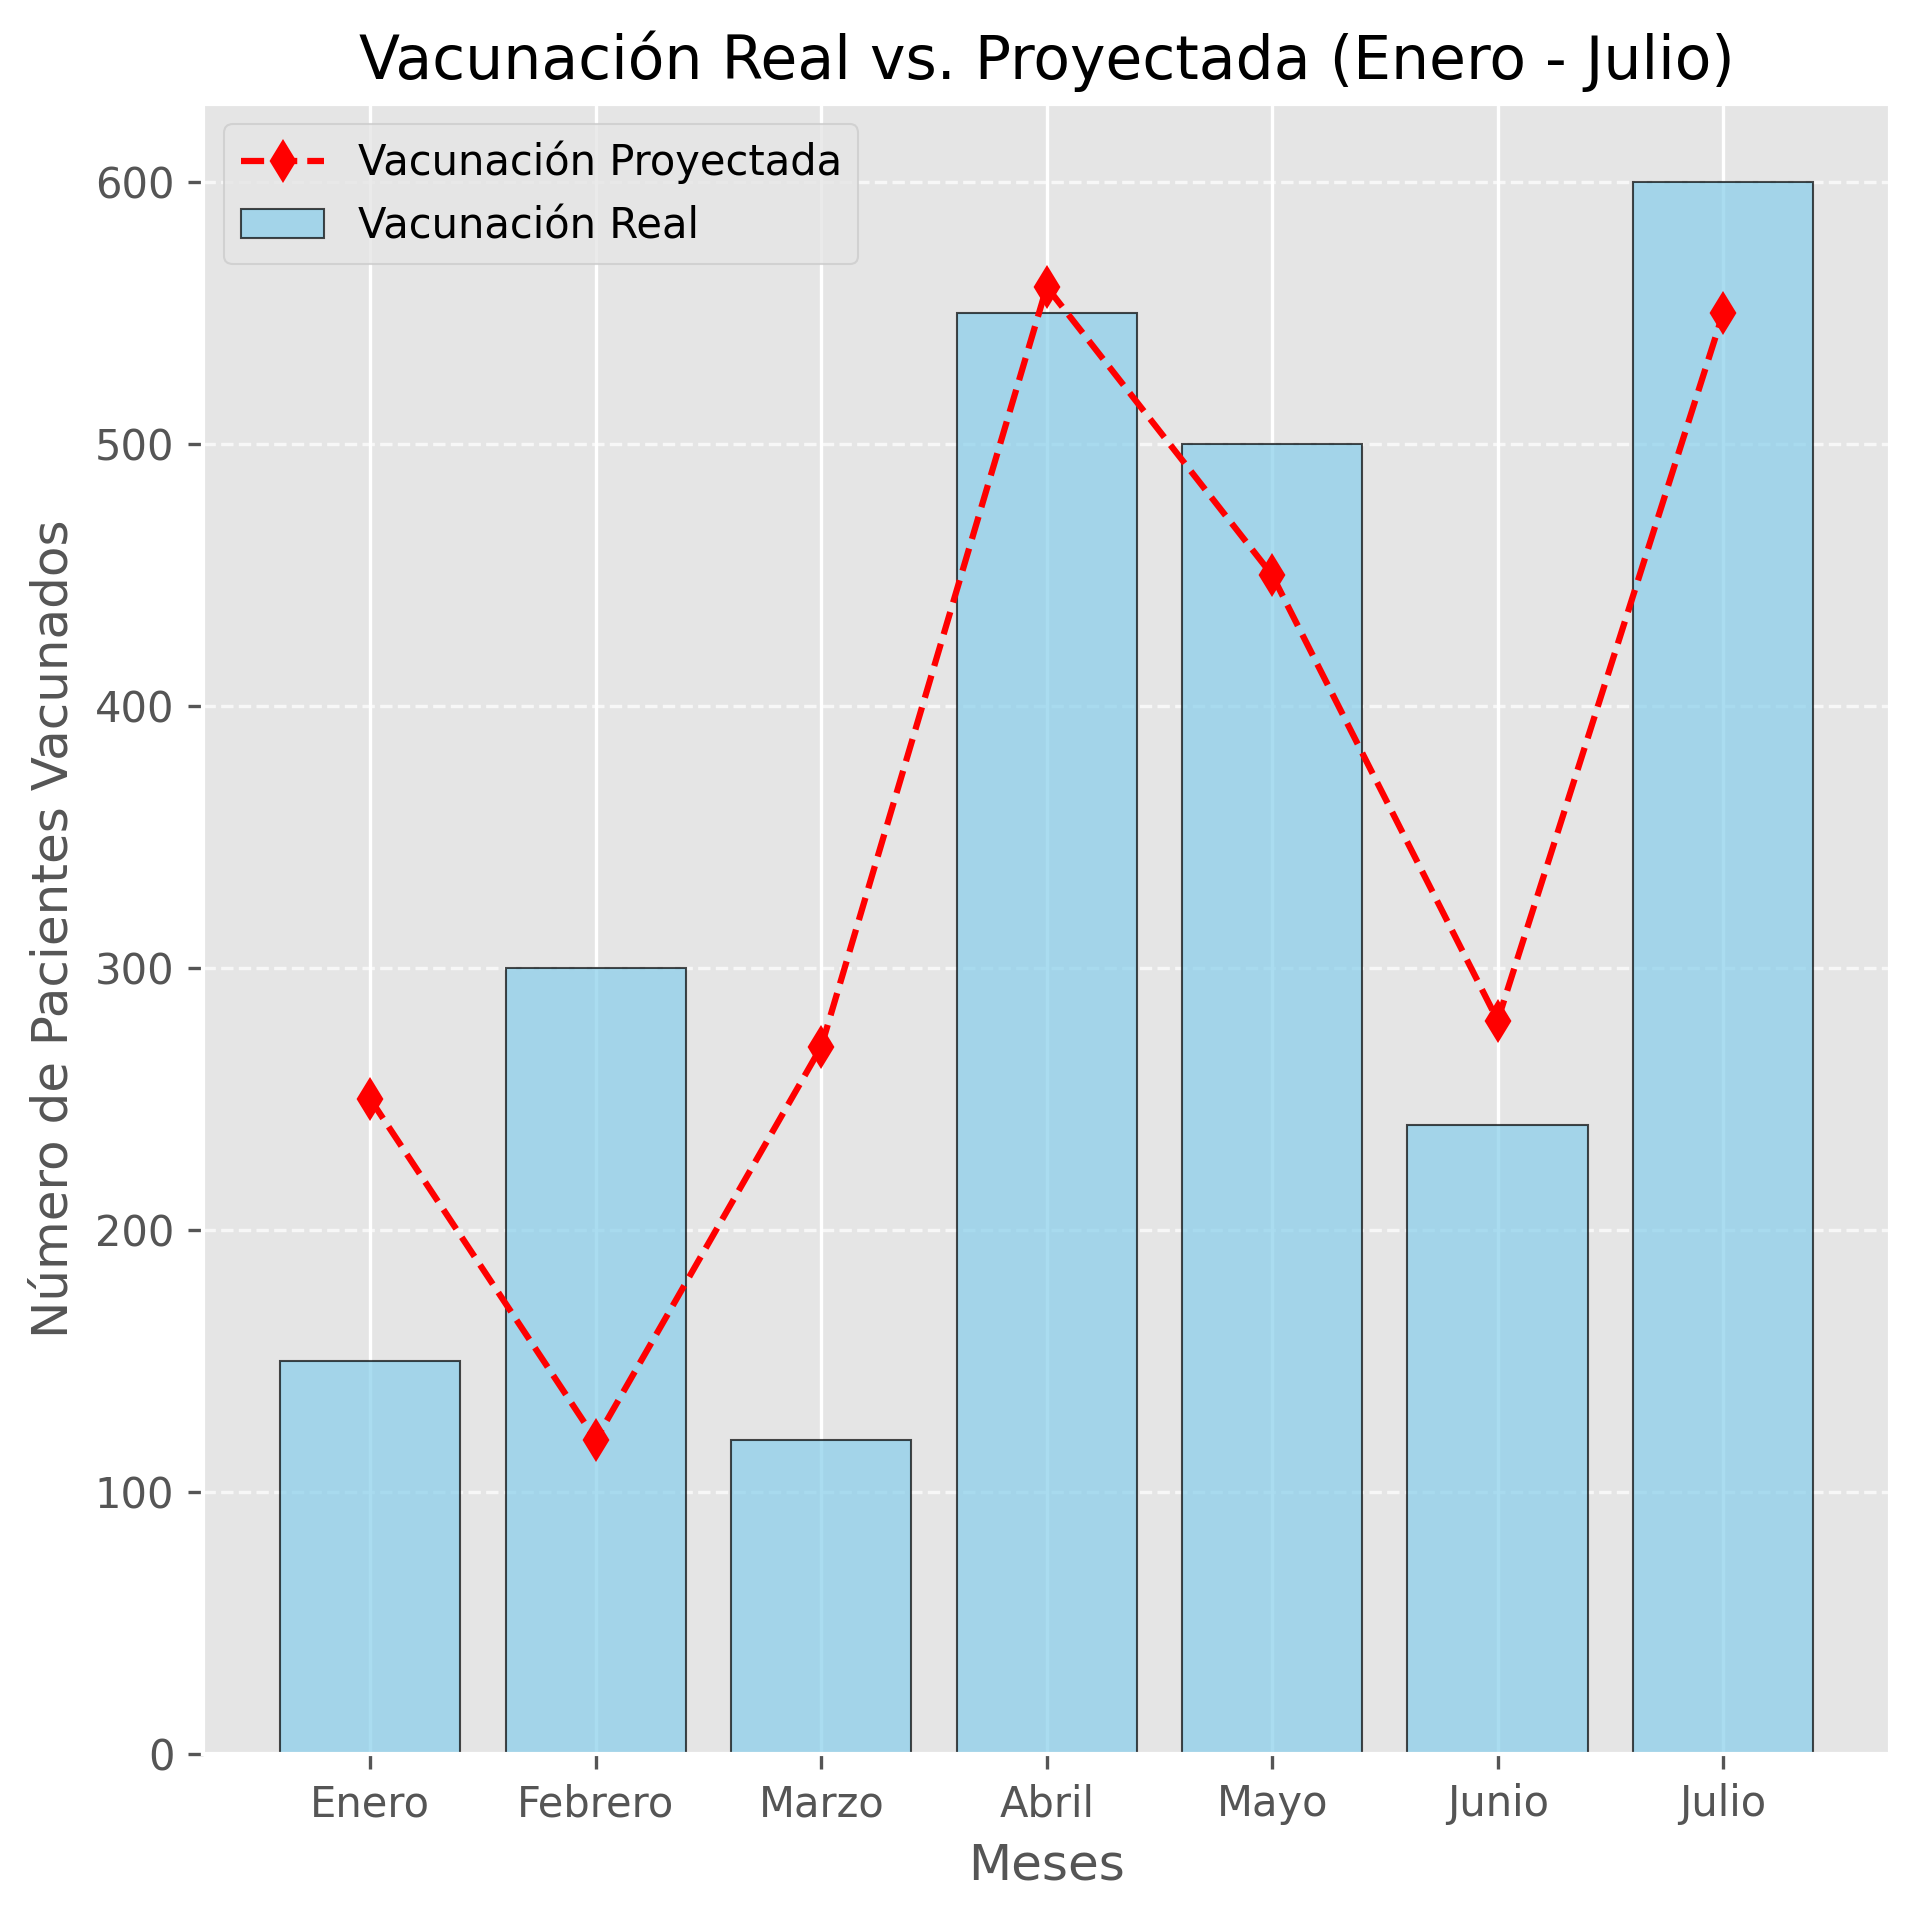
\includegraphics[keepaspectratio]{index_files/figure-pdf/cell-12-output-1.png}}






\end{document}
